\documentclass[11pt]{article}
\usepackage{amsmath,amsfonts}
\usepackage[numbers,sort&compress]{natbib}
\usepackage{times}
\usepackage[left=2.54cm,top=2.54cm,right=2.54cm,bottom=2.54cm,bindingoffset=0.0cm]{geometry}
\usepackage{setspace}
\usepackage{enumerate}
\usepackage{enumitem}
\usepackage{wrapfig}
\setcounter{secnumdepth}{0}
\usepackage{fullpage}
\usepackage{titlesec}
\titleformat{\section}{\large\bfseries}{\thesection}{1em}{}
\titleformat{\subsection}{\bfseries}{\thesubsection}{1em}{}
\usepackage{parskip} % skip paragraph indentations
\usepackage{lipsum}
\usepackage{hyperref}
\usepackage{graphicx}
\usepackage{amssymb}
\usepackage[x11names]{xcolor}
\usepackage{hyperref}
\usepackage{enumitem}
\usepackage{booktabs}
\usepackage{amsmath}
\usepackage{amssymb}
\usepackage{mathrsfs}
\usepackage{caption} \captionsetup[table]{singlelinecheck=false} %makes table captions left-justified
\usepackage{framed} % to add frames around comments
%\hypersetup{backref,colorlinks=false,
%    urlbordercolor=LightSkyBlue4,          % color of internal links
%    citebordercolor=SpringGreen4,        % color of links to bibliography
%    filebordercolor=magenta,      % color of file links
%    linkbordercolor=Red3, pdfborderstyle={/S/U/W 1.5}}
\newcommand{\Prob}[1]{\Pr{\left( #1 \right)}}
\newcommand{\q}[1]{``#1''} % easier way to get double quotes
\newcommand{\argmin}{\text{argmin}}
\usepackage{authblk} % for title page
\renewcommand\Affilfont{\fontsize{10}{10.8}\itshape}
\renewcommand\familydefault{\sfdefault} 
\usepackage{datetime2}
%\renewcommand{\dateseparator}{-}
\usepackage{atbegshi}% http://ctan.org/pkg/atbegshi -- removes blank page at start of doc
\AtBeginDocument{\AtBeginShipoutNext{\AtBeginShipoutDiscard}}
\setcounter{page}{0}

\lhead{Large groups and learning costs promote signal-based assessment} 


\begin{document}
\noindent
\title{Large groups and high learning costs promote the evolution of signal-based social assessment} 
\author{}
\date{} 
\maketitle

%New target journal: Proc B 
%instructions: http://rspb.royalsocietypublishing.org/author-information
% open access: https://royalsociety.org/journals/authors/open-access/

%%%%%%%%%%%%%%%%%%%%%%%%%%%%%%%%%%%%
\linenumbers

\section*{Lay summary}
%Animals that live in groups often need accurate information about their group mates, but there are several ways that this assessment can work. Some animals learn to recognize something about others, and sort individuals into categories or remember particular individuals, but others may learn general rules of thumb that apply to all individuals. We find that recognition learning is always more difficult than rule learning in large groups and when animals have poor memory. In these cases, it is better to learn about general rules of quality, rather than relying on learning about to recognize individuals.

% % TERMS:
% individual recognition vs signal-based assessment strategies
% categorical vs rule-based strategies for inferring quality from signal

% STYLE NOTES:
% - how to treat rule / rule of thumb?

%%%%%%%%%%%%%%%%%%%%%%%
\section*{Abstract}
%%%%%%%%%%%%%%%%%%%%%%%
%Animals in social groups benefit from having accurate information about their group mates. Different species have different methods for gathering this information: some animals recognize members of their groups as individuals, while others coarsely categorize conspecifics based on observable traits. In many animals, a property of interest, for example dominance or health, is correlated with an otherwise unimportant trait, which is then referred to as a badge of status. Much is known about the circumstances that promote the evolution of either individual recognition or a badge of status, but there are few studies that compare the effectiveness of the two systems of learning. In order to study how group size and cognitive abilities influence the effectiveness of both types of learning and to determine the circumstances under which one is preferable, we develop and analyze a simple model of an animal social group, in which animals learn by interacting with each other and by observing these interactions. Regardless of how the animals assess the quality of their group mates, we find that larger group sizes and longer memory windows make it easier to learn more accurately and more quickly. We also find that intermediate perceptive abilities maximize the effectiveness of learning about a badge of status and that observational learning is more beneficial for animals using individual recognition. Finally, we find that learning about a badge of status is less costly than individual recognition when animals live in large groups, have short memories, and have coarse perceptive abilities.



\textbf{Keywords:} badge, cognition, evolution, learning, recognition, signal, social groups

\newpage
%%%%%%%%%%%%%%%%%%%%%%%
\section*{Introduction} 
%%%%%%%%%%%%%%%%%%%%%%%
%% SOCIAL INFORMATION
Animals in social groups benefit from having accurate information about their group mates \citep{Seyfarth:2010bh}. For example, an animal can make a better decision about whom to fight if it knows something about the dominance ~\citep{Waal:1986ys,Cowlishaw:1990vn,Bergman:2003qf,Seyfarth:2005ve,Flack:2006uq,Hobson:2015uq} or resource holding potential~\citep{Rhijn:1980uq,Freeman:1985kl,Dick:1990cr,Lemel:1993ve,Part:1997ys} of the other members of its group. Conversely, knowledge about other animals' dominance can help an animal make decision about with whom to ally itself \citep{Engh:2005qp}. A female can  make a better decision about whom to mate with if she has some information about a male's likelihood of investing in parental care~\citep{Qvarnstrom:1997fk,McGlothlin:2007au,Olsen:2010uq} or his health~\citep{Folstad:1992kx,Loyau:2005nx}. In addition to affecting how animals make decisions about social interactions, the information that animals have about each other can affect the type of social structure that emerges in their group \citep{Dugatkin:2004hz,Hobson:2015uq,Brush:2018ss}. In order to understand the evolution of sociality, it is therefore important to understand how animals makes assessments of each other and strategies for doing so evolve.  

%% SIGNAL-BASED ASSESSMENT
One class of strategies for making social assessments is based on signals. There are many examples of species in which one trait acts as a signal of another less visible trait. When the property of interest is an animal's resource holding potential, the signal is called a badge of status \citep{dawkins1978signals,Rohwer:1981vn,Rohwer:1982fk,Ripoll:2004vn,sheehan2016evotradeoff}. A classic example of this is provided by house sparrows (\emph{Passer domesticus}), in which the size of a male's bib is correlated with his dominance \citep{Veiga:1993fk,Veiga:1995ys}. Badges of status have also been demonstrated in several other species of birds (e.g., \citep{Remy:2010fk,Olsen:2010uq,Lemel:1993ve,Tibbetts:2009kx}), mammals (e.g., \citep{Gerald:2001zm}), reptiles (e.g., \citep{Fox:1990hd}), and insects (e.g., \citep{Tibbetts:2004kx}). Signals can also provide information about other properties. For example, some species of birds have signals that communicate their current health status \citep{Folstad:1992kx,Loyau:2005nx}. In humans, a smile may be a signal of a person's likelihood of cooperating \citep{Schug:2010be}. Once such a signal has evolved, animals can use the signals displayed by their peers to make estimates of the property of interest, be it resource holding potential, health, likelihood of cooperating, or anything else.

It is difficult to determine how animals actually use a signal to assess conspecifics. In order to prove that a trait is a quality signal, scientists usually identify a statistically significant linear relationship between the putative signal and a property of interest (e.g., \citep{Rohwer:1981vn,Rohwer:1982fk,Ripoll:2004vn,Tibbetts:2004kx}). Animals could use such a linear relationship as a rule dictating how to map a signal to a quality value. While it is often assumed that animals are born knowing this rule, it is also plausible that they learn it over the course of interacting with conspecifics. Many cognitive processes in both humans and non-human animals are based on a categorical perception of the world \citep{Harnad:1990ux}. Both sound (e.g., \citep{Wyttenbach:1996wj,Nelson:1989rt}; reviewed in \citep{Bornstein:1987ec,Ehret:1987jh}) and color (e.g., \citep{Lim:2016ye}; reviewed in \citep{Bornstein:1987ec}) have been demonstrated to be perceived categorically by different types of animals. Categorization provides an alternative way for animals to make inferences about the quality of their peers based on the signals they display. For example, a zebra finch might categorize conspecifics by whether their bills are more red or orange and subsequently learn that birds with red bills have high resource holding potential and birds with orange bills have low resource holding potential TKTK.   
 
%% INDIVIDUAL RECOGNITION
In contrast to using signals to assess one's peers, an animal can simply recognize and learn about each other animal individually. Individual recognition has been demonstrated in many species and can be based on visual, olfactory, or auditory traits (reviewed in \citep{Tibbetts2007IndividualDifferent}). An animal with imperfect cognitive abilities may confuse similar conspecifics. As an animal's ability to discriminate becomes worse, it will confuse more and more animals and may resort to learning about them categorically. Individual recognition can therefore be thought of as extremely fine categorical recognition \citep{Barnard:1979fk}. Such a spectrum from coarse-grained to fine-grained perceptive abilities has actually been demonstrated within the group of paper wasps: some species distinguish between other wasps based on the number of black patches on their face, a relatively coarse trait \citep{Tibbetts:2004kx}, whereas in other species, wasps can recognize specific individuals based on their unique facial patterns \citep{Tibbetts:2002ys}. 

%% BIG UNKNOWN QUESTION
Regardless of how the assessment is being made, there are two things that have to be present in order to have a functional system of social assessment: (1) a trait that is used as either a quality signal or an identity signal and (2) an assessment strategy that is either signal-based or recognition-based.  On the signal side, much work has been done to understand when quality signals or badges of status should be expected to evolve (e.g., \citep{Whitfield:1987tg,Rohwer:1975fk,Rohwer:1982fk,Dawkins:1991ly,Johnstone:1995vn,Lachmann:1998fk,Tibbetts:2009kx}). For example, in birds, badges of status seem to evolve in species that live in large and fluid groups in the non-breeding season \citep{Tibbetts:2009kx}. There are also many studies that have identified the circumstances that facilitate the evolution of identity signals \citep{Rohwer:1975fk,Whitfield:1987tg,Sheehan:2009we,Pollard:2011te,Sheehan:2014fk}. In particular, identity signals are more likely to evolve in species that have complex social structures or highly territorial behavior \citep{Tibbetts2007IndividualDifferent}. On the assessment side, we do know some factors that should facilitate the evolution of individual recognition. For example, there needs to be sufficient variability in the trait that will be used as an identity signal \citep{Sheehan:2014fk}. Individual recognition is also more likely to evolve in species where animals can avoid costly fights by recognizing which conspecifics to avoid \citep{DEttorre:2005nu}.  \citet{sheehan2016evotradeoff} pursued a thought experiment in which they compared the errors and learning time associated with quality signaling and individual recognition and made predictions about when one or the other would be preferable. They predicted that signal-based assessment strategies will not be affected by the number of interactions a pair of animals engages in or the size of the social group, whereas individual recognition should improve over time and become more difficult in larger groups \citep{sheehan2016evotradeoff}. They also predicted that individual recognition should be preferable in small groups when animals have many opportunities to learn about each other \citep{sheehan2016evotradeoff}. Quantitative support of these qualitative predictions was left for future work. Despite the fact that \citet{sheehan2016evotradeoff} identified this as an important problem, there are few modeling studies that compare the efficacy of signal-based assessment to that of individual recognition. 

%%MEMORY
Whether a signal-based or recognition-based assessment strategy is preferable will depend on several factors. As we described above, individual recognition can only work if the animals have sufficiently fine perceptive abilities. There are other cognitive constraints that are important for understanding which type of assessment method is best. An animal's memory can limit its ability to remember its assessments of its peers. 
If animals use a linear rule to make assessments about their peers, there are essentially two parameters to remember: the slope and intercept of the line. Similarly, if animals categorize their peers, they only have to remember as many pieces of information as there are categories. However, if animals use individual recognition, they must remember the quality of each of their peers, which can become prohibitively difficult in large groups  \citep{Rohwer:1982fk,Solberg:1997uq}. It can become even more problematic if animals have to remember the relationships between pairs of other animals ~\citep{Seyfarth2015SocialCognition}. Even humans are thought to be limited in terms of the number of people we can recognize. Previous work has hypothesized that humans can only remember the faces of about 150 people \citep{Dunbar:1993zr,Hill:2003ly}, which may have limited group size over the course of human evolution~\citep{Dunbar:1992ys,Dunbar:1993zr}. 

%%UTILITY OF ASSESSMENT
The final factor in understanding when which type of assessment will evolve is being able to quantify the costs and benefits of using either strategy. Animals assess each other and use information about their group mates to decide how to interact with them in the future. Therefore, if animals learn about each other inaccurately, they will make inappropriate decisions and incur costs. On the other hand, individuals are constrained in the total amount of effort and time that they can devote to assessing each other \citep{MacIver:2010ve}. Additionally, if interactions are aggressive, engaging in more interactions than necessary can lead to injury. The overall cost of using a particular assessment strategy will be a combination of the costs of the errors made and the time it took to make the assessment. There is an inherent tradeoff between accuracy and speed because waiting longer and gathering more information improves the accuracy of an animal's assessment.  This tradeoff will vary from species to species and will affect which assessment strategy is preferable.  

Our goal in this paper is to understand when different types of assessment strategies will evolve by comparing the costs of signal-based assessment strategies and individual recognition.  In order to do so, we developed an agent-based model of an animal social group in which animals assess each other's quality through dyadic interactions and incur costs based on these assessments. We first analyze how group size, cognitive abilities, and the cost of the time spent assessing influence each assessment strategies. We then identify the cognitive traits that optimize an animal's ability to assess its peers via categorical and individual recognition. Finally, we identify the circumstances under which each strategy is preferable. In general our results conform to the predictions of \citet{sheehan2016evotradeoff}, although we extend their thought experiment by analyzing both innate \emph{and} learned signal-based assessment strategies and considering a categorical assessment strategy that grades into individual recognition. 
 

%%%%%%%%%%%%%%%%%%%%%%%
\section*{Model } 
%%%%%%%%%%%%%%%%%%%%%%%

%\subsection{Interactions and quality assessment}
We consider with a group of animals containing $N$ individuals (see Table~\ref{tab:vars} for parameter descriptions). We assign each animal a quality value, $q_i$, and a signal, $s_i$. Quality can be thought of, for example, as fighting ability, resource holding potential, body size, body condition, or any other property about which it would be beneficial to have accurate information and which it may be difficult to estimate without interacting with an animal. While the types of traits that can be used either as quality signals or for individual recognition are likely different \citep{Dale:2001dv}, we assume that the animals vary in a single visible trait, which can be used either as a quality signal or for individual recognition and which can be measured without having to interact with an animal.  

Specifically, we draw quality values $\{q_1,\dots,q_N\}$ from a normal distribution with mean $0$ and standard deviation $\sigma_\text{q}$. We then generate $N$ signal values $\{s_i\}$ such that 
%$\min_i{s_i}\approx -1$, $\max_i{s_i}\approx 1$, and 
$\max_i\{s_i\}-\min_i\{s_i\}=2$ and the sample correlation between $\{q_i\}$ and $\{s_i\}$ is precisely $\rho$. 
The higher $\rho$ is, the more informative the signal is about the underlying quality of the animals. The animals then use these signals to assess the quality of their group mates.

We consider two main ways in which animals assess each other: (1) a linear rule that maps signal to quality, which can be either innate or learned, and (2) categorization, which becomes into individual recognition when the animals can perceive small enough differences to be able to distinguish all of their peers. Under each system, the animals interact and assess each other for $T$ timesteps. At each point in time, two animals, $i$ and $j$, are chosen randomly to interact. Through this interaction, each receive noisy information about the other's quality: $i$ perceives $j$'s quality to be $\hat{q}_j=q_j+\xi$, where $\xi$ is drawn from a normal distribution with mean $0$ and standard deviation $\sigma_\xi$.  Additionally, every animal makes an assessment of every other at each point in time. We will write $a_{ij}(t)$ for the assessment that animal $i$ has of animal $j$ at timestep $t$. We now describe each assessment strategy system in detail.

%XXX MOVE TO DISCUSSION
Observational learning is known to be important in many systems (e.g., \citep{Freeman:1985kl,Holekamp:1991nx,Schaik:2011oq,Hobson:2015uq,Seyfarth2015SocialCognition}). However, we are interested in the inherent costs and benefits of the different assessment strategies and do not consider observational learning here. 


\subsection*{Linear rule}
We first describe animals that use a linear rule to infer quality from signal. In this case, each animal's assessment is given by
\begin{equation*}
a_{ij}(t)=m_i(t)s_j+b_i(t),
\end{equation*}
where $m_i(t)$ and $b_i(t)$ are the slope and intercept that $i$ believes describe the linear relationship between signal and quality at timestep $t$. When the rule is innate, these parameters do not change over time and they are the same for all animals in the group. An innate rule has presumably evolved over time to describe the average relationship between signal and quality. To model this, we generate $10,000$ groups with quality and signal values as described above. In each group, we find the slope $m$ and intercept $b$ of the best-fitting line through the points given by $\{s_i\}$ on the x-axis and $\{q_i\}$ on the y-axis. We then take the average of these over all $10,000$ groups and assume that all individuals in the group use $m_i(t)=\bar{m}$ and $b_i(t)=\bar{b}$ for all $i$ and all $t$. Thus, there is no learning and animals can use this rule immediately. 

%\subsection*{Learned rule}
We also allow animals to learn a rule to assess each other's quality. In this case, all members of the group are initially naive and have no estimate of the slope and intercept of the signal-quality relationship. The animals have a ``memory window" $w$ such that each animal remembers any interactions that have occurred within the last $w$ timesteps. From each of these recent interactions, an animal $i$ stores the signal of its opponent, $s_j$, as well as noisy information about its quality, $\hat{q}_j$.  Then $m_i(t)$ and $b_i(t)$ are the slope and intercept from the best-fitting line through the points given by the observed $\{s_j\}$ on the x-axis and the observed $\{\hat{q}_j\}$ on the y-axis.   

\subsection*{Categorization}
We next describe animals that perceive their conspecifics' signals categorically. In this case, the way animals categorize their peers depends on the magnitude of the differences in signals they can perceive. Specifically, an animal can only distinguish between two other animals $j$ and $k$ if $|s_j-s_k|>\delta$, that is, if their signals are sufficiently different. If the animals have fine perceptive abilities, the parameter $\delta$ will be small, and if the animals have coarse perceptive abilities, the parameter $\delta$ will be large. For example, if $\delta$ is be large, an animal can only discriminate among animals with small, medium, and large signals, and the best it can do is to learn about the quality of all animals in each of these three categories. On the other hand, if $\delta=0$, an animal can discriminate among every individual in its group and is capable of individual recognition. We will refer to the strategy of using categorization with $\delta=0$ as individual recognition below.

Before any interactions take place, each animal in the group divides its peers into categories. It does so by picking another animal, $j$, at random. All animals whose signals are within $\delta/2$ of $s_j$ are put in the same category. Then the focal animal picks an uncategorized animal at random, $k$, forming a second category of all uncategorized animals whose signals are within $\delta/2$ of $s_k$. The process continues until every animal in the group has been assigned a category. The parameter $\delta$ can therefore be thought of as ``category width."  Different animals will categorize the group differently and may perceive different numbers of categories. Figure \ref{category_diagram} shows one example of this process for various values of $\delta$. Because we analyzed the effects of several parameters, we chose a representative set of values rather than exploring every possible value of each parameter. In particular, we allow $\delta$ to take on the values $0$, $0.25$, $0.5$, $0.75$, and $1$.

%\subsection*{Updating assessments}
As with the learned rule above, at first, the group consists entirely of naive animals: at $t=0$, no animal has an opinion of any other. Again, each animal has a memory window $w$ such that it remembers categories it has encountered in the last $w$ timesteps and forgets its opinion of categories it has not interacted with so recently. Each animal then updates its assessment of the other to be the weighted average of its old estimate and the new information it has received. Specifically, if $i$ already has an assessment of $j$'s category, its new assessment of the category
\begin{equation*}
a_{ij}(t+1)=(1-r)a_{ij}(t)+r\hat{q}_j,
\end{equation*}
where $r$ is the ``updating rate" describing how much each animal changes its assessment based on the interaction. As with $\delta$, we choose a representative set of values of $r$ to explore, specifically, $0.05$, $0.1$, $0.25$, and $0.5$. Animal $i$ simultaneously updates its opinions of all the other animals in the same category as $j$.
If $i$ has not previously interacted with animals in $j$'s category or if $i$ has forgotten about the category, its new estimate of the category is
\begin{equation*}
a_{ij}(t+1)=r\hat{q}_j.
\end{equation*}
%In words, an animal's baseline opinion of a stranger is $0$, the average quality value of any group. 

When $\delta=0$, there are as many ``categories" as there are animals and the animals can be said to be using individual recognition. As category width increases, the average number of categories animals recognize decreases (Figure \ref{category_diagram}). According to \citet{sheehan2016evotradeoff}, what distinguishes an assessment strategy that relies on quality signals from individual recognition is that, with a quality signal, an animal can know something about a conspecific based solely on the signal it displays without having had to interact with it. In our model, this is true for animals using categorization with category width $\delta>0$, as well as for animals using either an innate or learned rule (Figure \ref{schematic}). In other words, both the categorization and rule strategies we analyze can be considered signal-based assessment strategies that differ in whether they are innate or learned and in how animals infer quality from signal. 
 
\subsection{Assessment errors }
For each assessment system and each combination of parameters, we simulate $25$ groups undergoing the processes just described.  To quantify how well the animals assess each other, we measure how accurately and how quickly they assess each other's quality. The error of animal $i$'s assessment of animal $j$ at time $t$ is $e_{ij}(t)=|a_{ij}(t)-q_j|$. For a given combination of parameters, we take the average error that any animal makes in its assessments of the rest of its group over all groups, 
\begin{equation*}
\epsilon(t) = \frac{\sum_{\text{groups}}\sum_i\sum_{j\in \mathscr{O}_i(t)}e_{ij}(t)}{25N|\mathscr{O}_i(t)|},
\end{equation*}
where $\mathscr{O}_i(t)$ is the set of animals about whom $i$ has an opinion at time $t$.

In Figure \ref{tradeoff} we show representative examples of how the average error of animals using each assessment system changes over time.  For animals using either a learned rule or categorization, as the animals learn about each other, $\epsilon(t)$ decreases until it reaches an asymptote (Figure \ref{tradeoff}). At first, animals are more or less guessing about the quality of their peers, which results in a high average error. When learning is difficult, for example because the animals' memory is poor or there are many animals to learn about, the average error barely decreases from its initially high level (Figure \ref{tradeoff}). When learning is easier, for example because the animals can remember more interactions, because there are fewer animals to learn about, or because the signal becomes more informative, average error decreases over time and can even approach $0$ (Figure \ref{tradeoff}).  

\subsection{Assessment costs }
We are interested in identifying which assessment strategy is least costly, as this is the strategy we might expect to evolve. To do so, we must measure the cost associated with each assessment strategy. Animals incur costs when they have inaccurate estimates of their peers' quality and by continuing to spend time learning about each other when they could be engaging in other activities. We thus quantify the cost of learning at time $t$ as 
\begin{equation*}
C(t) = 2c\epsilon(t) +(1-c)\frac{t}{T}.
\end{equation*}  
The parameter $c$ ranges from $0$ to $1$ and quantifies the tradeoff between accuracy and speed: when $c$ is close to $1$, errors are more costly and when $c$ is close to $0$, the time spent learning is more costly. The factors of $2$ and $1/T$ ensure that the two costs are on the same scale, namely between $0$ and $1$. 
The cost function initially decreases, reaches a minimum, and either stays constant at that value or starts to increase (Figure \ref{tau}). 

As we will show, increasing an animal's memory always improves how accurately it can learn. However, it may be costly to invest in improved memory. Rather than using an arbitrary cost function to describe these costs and finding the optimal memory window, we treat memory window as a variable that affects how well the animals can learn and what learning strategies they should use. 
%As we show later, it is sometimes beneficial for an animal to group its peers into categories based on the signals they display. Similarly, different updating rates are beneficial in different circumstances.

\subsection{Optimization }
There are strategies animals can use to minimize their costs within a particular assessment strategy. In order to study the evolution of the assessment strategies more broadly, we first study the evolution of each assessment strategy individually. While group size $N$ and signal-quality correlation $\rho$ may evolve over time, we assume that they are fixed on the timescales we consider. Similarly, memory $w$ may evolve over time, but we consider it as a fixed parameter in order to analyze the effects of memory on the evolution of assessment strategies. 

One strategy that animals \emph{can} vary is how many interactions they engage in before they stop learning. The animals should stop interacting for the sake of learning when the cost function $C(t)$ first reaches its minimum value (Figure \ref{tau}). We refer to the number of interactions at which this occurs as the stopping time $\tau$. In other words, $C(\tau)$ is the minimum cost that can be incurred for a given set of parameters. When $c$ is close to $1$, the animals will keep learning to improve their accuracy and $\tau$ will be high, whereas when $c$ is close to $0$, taking time to learn is costly and $\tau$ will be low. For animals using an innate rule, $\tau$ is always equal to $1$ because they do not engage in learning and cannot improve their assessments by engaging in more interactions. 
% QUESTION: above, should the "c" be upper or lowercase here? "which is the number of interactions it takes before $C$ first reaches its minimum value" (was upper, but I think it should be lower??) 
% ANSWER: in that case it should be C, the cost function itself
% Memory is also costly 

Animals using categorization may also be able to evolve or optimize the values of $\delta$ an $r$ to minimize their costs. We first fix the group size $N$, signal-quality correlation $\rho$, memory window $w$, and cost of errors $c$. Then, for every combination of $\delta$ and $r$ we find the stopping time $\tau$ and therefore the minimum possible cost $C(\tau)$. Finally, we find the combination of $\delta$ and $r$ that minimizes $C(\tau)$. These are the parameters we would expect to evolve in a population using categorization as its assessment strategy. 

To compare all assessment strategies, for a given group size $N$ signal-quality correlation $\rho$, memory window $w$, and cost of errors $c$, we compare the cost of learning for animals using an innate rule ($C(1)$, which does not depend on $w$), for animals using a learned rule ($C(\tau)$), and for animals using categorization ($C(\tau)$ with optimized $\delta$ and $r$). We would expect that the assessment system with the lowest cost would invade a population using either of the other two systems.

%There are six important parameters in our model: group size $N$, the correlation between signal and quality $\rho$, memory window $w$, category width $\delta$, updating rate $r$, and stopping time $\tau$.  

The entire model was written in R and all model code will be released on publication on Github.

%%%%%%%%%%%%%%%%%%%%
\section*{Results}
%%%%%%%%%%%%%%%%%%%%
\subsection*{The effects of the signal-quality correlation, group size, and cognitive abilities on learning}
We first analyze how stopping time ($\tau$)  and average error ($\epsilon(\tau)$) depend on various parameters describing the animals' learning strategies, group demographics, and cognitive abilities. Recall that stopping time ($\tau$) is the number of interactions at which the animals' overall cost $C(t)$ stops decreasing and $\epsilon(\tau)$ is the average error of the animals' assessments at that point in time. Additionally, when time is not at all costly ($c=1$), the overall cost is equal to twice the animals' average error ($C(\tau)=2\epsilon(\tau)$).

Updating rate ($r$) and category width ($\delta$) only affect animals using categorization. (Recall that categorization becomes recognition when category width $\delta=0$.) The effects of the two parameters are similar: with higher updating rates and larger category widths, the animals gather information more quickly, but that information is noisier, either because more weight is given to the animals' noisy observations or because more animals are lumped together into the same category. Therefore, as either updating rate or category width is increased, the average error of the animals' assessments plateaus more quickly and stopping time decreases (Figure \ref{tradeoff}). When the animals have long memories, this is associated with an increase in the equilibrium level of error (Figure \ref{tradeoff}A and C). However, when the animals have short memories, this decrease in learning time is associated with an \emph{decrease} in the equilibrium level of error as well (Figure \ref{tradeoff}B and D). In other words, when the animals have short memories, it is beneficial to gather as much information as quickly as possible, even if that information is noisier. This shows that using categorization ($\delta>0$) can be preferable to using recognition ($\delta=0$) under some circumstances. (The interactions between memory window, category width, and updating rate are shown in full in Figure \ref{interactions}.)

The signal-quality correlation ($\rho$) only affects animals using signal-based assessment strategies, i.e. either type of rule or categorization with $\delta>0$, but not recognition. Signal-quality correlation does not have a strong effect on how long it takes to assess one's group mates (Figure \ref{parameters}A), but increasing the correlation dramatically reduces the errors made by animals using signal-based assessment strategies (the blue and purple curves in Figure \ref{parameters}E).

As group size increases ($N$), it takes animals longer to learn about their peers (Figure \ref{parameters}B). (Remember that animals using an innate rule do not learn and their stopping time is essentially always equal to $1$.) As group size increases, animals using categorization or recognition make greater errors (red and purple curves in Figure \ref{parameters}F), but the error of animals using either type of rule is not strongly affected (the blue curves in Figure \ref{parameters}F).

The animals' memory window ($w$) really only affects animals using categorization and recognition. For these animals, as memory window increases, it takes longer their assessment error to reach a plateau, so stopping time increases (red and purple curves in Figure \ref{parameters}C). But because they can remember more information, their errors are reduced (red and purple curves in Figure \ref{parameters}G). As the cost of errors ($c$) increases, animals using any learned strategy should invest more time in learning (Figure \ref{parameters}D), which helps them reduce their errors (Figure \ref{parameters}H). The interactions between the effects of signal-quality correlation, group size, memory window, and cost of errors on stopping time and average error are shown in Figure \ref{time} and \ref{error}. In summary, signal-quality correlation ($\rho$), the effects of group size ($N$), memory window ($w$), and cost of errors ($c$) on learning speed and learning accuracy are generally as expected and confirm that our model is a reasonable description of some of the basic properties of a real social system. 
  
\subsection*{Optimal learning strategies for animals using categorization}
We are interested in determining when we would expect signal-based assessment strategies, as opposed to recognition, to evolve. To this end, we first compare the strategies of categorization ($\delta>0$) and recognition ($\delta=0$). As described above, for each signal-quality correlation ($\rho$), group size ($N$), memory window ($w$), and cost of errors ($c$), we find the stopping time ($\tau$), updating rate ($r$), and category width ($\delta$) that minimize the cost of using categorization. If these strategies were allowed to evolve, within a population using categorization, then we would expect them to evolve toward these optima. Remember that the overall cost of using a strategy is a weighted average of the error with which animals can assess their peers and the number of interactions it takes to reach an accurate assessment and that the cost of errors reflects the importance of making accurate assessments of one's peers. 

Using recognition is only a better strategy (i.e. less costly) than recognition when the signal is very highly correlated with quality ($\rho=0.99$) (Figure \ref{opt_delta}). When $\rho=0.99$, recognition is better when the animals have short memories and when errors are not very costly (Figure \ref{opt_delta}). Under these circumstances, using a category width greater than $0$ helps the animals learn more quickly. Note that a category width greater than $0.25$ is never optimal: increasing $\delta$ beyond $0.25$ only makes the animals' learning process noisier. As group size increases, memory window and the cost of errors do not need to be very low before categorization becomes preferable (Figure \ref{opt_delta}). In summary, rather than focusing on the individual identity of their peers, the animals should categorize the rest of their group based on the signals they display and assess all of the animals in each category simultaneously, when the animals live in larger groups, when they have with short memory windows, and when errors are not very costly. Conversely, animals should invest in individual recognition when the signal-quality correlation is lower, when they live in smaller groups, when they have long memory windows, and when errors are costly. 

For those parameters where categorization ($\delta=0.25$) is optimal, it is optimal to use a high updating rate (Figure \ref{l}). In fact, the optimal updating rate behave similarly to the optimal category width: a high updating rest is best when the animals live in larger groups, when they have short memory windows, and when errors are not very costly, and  (Figure \ref{l}). When animals use optimal strategies---stopping time, updating rate, and category width---the error with which animals assess their peers increases as memory window decreases, as the cost of errors decreases, and as group size increases (Figure \ref{error}). 

%For animals using a learned rule, the optimal stopping time depends on their memory window and the cost of errors (Figure \ref{time_rule}), but the errors with which they learn stays relatively constant (Figure \ref{error_rule}).  

\subsection*{Optimal assessment strategy}
Having found the optimal parameters for animals using categorization, we can now compare the overall costs of using each of the three assessment strategies. We imagine that evolution \emph{within} the categorization system is more likely and that it is likely to occur on a faster timescale, so that categorization would be optimized before a learned or innate rule would arise.  Thus, by comparing the costs of the optimized categorization strategies to the costs of using either a learned or innate rule, we can find which strategy would be expected to evolve.

When we compare all three assessment strategies, we find that recognition is the best strategy in small groups, when animals have long memories, and when errors are costly (Figure \ref{best}). Note that the regions of Figure \ref{opt_delta} where $\delta=0.25$ is optimal fall in the regions of Figure \ref{best} where a rule is optimal. In other words, there are no parameters where categorization ($\delta>0$) is the best strategy of all (Figure \ref{best}).  Of the parameters where a rule is preferable, a innate rule is preferable to a learned rule only when group size is large ($N=100$) and the memory window is very short ($w\leq500$) (Figure \ref{best}). There are large regions of parameter space where all three assessment strategies perform almost equally (the grey regions in Figure \ref{best}). If we only compare the strategies that involve learning---categorization / recognition and the learned rule---our findings are similar: individual recognition is preferable in small groups, when animals have short memory windows, and when errors are costly (Figure \ref{comparison}).
%This agrees with predictions made by Sheehan et al. Whether learning about categories or a rule is easier is left for future research.

%%%%%%%%%%%%%%%%%
\section*{Discussion}
%%%%%%%%%%%%%%%%%
%to put somewhere: 
We find that the how strongly the signal is correlated with the property of interest determines whether a learned or innate rule is better. Whether animals use a learned or innate strategy for inferring quality from signal can in turn affect the evolution of the signal itself \citep{Kamo:2002vi}. A complete understanding of the evolution of social assessment will require considering the full feedback loop, that is including both the effect of the signal on the evolution of the assessment strategy and the effect of the assessment strategy on the evolution of the signal.


% Study question, restated/reframed
In animal social groups, having an accurate opinion about the quality of one's group mates is important in many contexts. One way that animals share information about their own quality is through a signal. There have been many studies about the evolution of badges of status, but the evolution of signal-based assessment strategies is less well studied. Here, we modeled quality assessment in social groups, with animals using either a signal, which allows them to infer the quality of an unknown animal, or individual recognition, which allows them to learn about each particular individual. We considered three signal-based assessment strategies: an innate linear rule mapping signal to quality, a learned rule, and categorization of signals. Our goal was to better understand the costs and benefits of each system and the conditions under which each system might be favored. 

In order to show that a particular trait in a particular species is being used as a badge of status, scientists usually identify a correlation between the trait and another property of interest and, ideally, also show that the animals themselves use the badge when they make decisions about how to interact with conspecifics. In the literature about badges of status, scientists make distinction between animals that use badges to asses their conspecifics and those that use individual recognition. The actual strategy that animals use to infer quality from a badge is usually ignored, or, if it is considered at all, it is often assumed that animals are born with an innate sense of how to interpret a badge of status. However, as we show, there are multiple ways of using a badge of status to infer quality and different strategies are preferable in different circumstances. This highlights the need for careful and clever empirical work that can uncover which strategy animals actually use. %citations in this paragraph TKTK XX XX ?? 

\subsection*{The effect of group size and cognition on learning} 

First, we evaluated how various demographics and cognitive traits affect the efficacy of each strategy in isolation. Both living in a large group and having a short memory make it more difficult to accurately assess one's group mates. Group size and memory affect all the assessment strategies that involve learning---a learned rule, categorization, and recognition---but they affect recognition most severely. We also find that agents using a signal-based assessment strategy learn more quickly and accurately when there is a strong correlation between the signal and quality. 
%While the correlation values we use are higher than those estimated in species for which this data has been collected (e.g., paper wasps \citep{Tibbetts:2004kx}, house sparrows \citep{Veiga:1993fk}, swamp sparrows \citep{Olsen:2010uq}, see Table \ref{corr_examples} for details), our model shows that even with a moderate correlation the badge system is an effective way to learn about one's group mates. 

Our model was inspired by the thought experiments carried out by \citet{sheehan2016evotradeoff}. They compared recognition with a signal-based assessment strategy, but did not specify exactly how the signal-based assessment strategy would work. They made four qualitative predictions to which we can compare our quantitative results. First, they predicted that animals using recognition should increase their accuracy over the course of interacting with their peers, whereas the accuracy of an animal using a signal-based assessment strategy should stay relatively constant over time (their Figure 1b). This is generally what we find, with the exception that animals using categorization, a signal-based assessment strategy \emph{can} dramatically improve their assessments over time (our Figure \ref{tradeoff}). Second, they predicted that the animals' accuracy should decrease dramatically as a function of group size for animals using recognition, but should be unaffected by group size for animals using a signal-based assessment strategy (their Figure 1c). This agrees with our findings (our Figure \ref{parameters}F). Third, they predicted that the ``cost" of learning should increase as a function of group size for animals using a signal-based assessment strategy, but should be unaffected by group size for animals using a signal-based assessment strategy (their Figure 1d). \citet{sheehan2016evotradeoff} considered costs that the animals incur from spending time learning about each other, as well as from investing in cognitive capacity. We do not consider the latter because there is little empirical evidence for the actual costs of memory and perception. The costs that they considered are therefore most similar to our stopping time. We find that group size dramatically increasing stopping time for animals using either recognition or categorization (our Figure \ref{parameters}B). This shows that group size can strongly affect the cost of using a signal-based assessment strategy, contrary to their prediction. Even though categorical perception has been documented in many species of animals, it is not usually considered in the literature on badges of status. By considering it here, we have shown that the specific strategy used to infer quality from a signal can lead to somewhat surprising results. Last, they wrote that there are ``conditions under which the reliability of quality signals and social recognition are expected to be similar" \citep{sheehan2016evotradeoff}. We found large areas of parameter space in which recognition, a learned rule, and an innate rule performed essentially equivalently (our Figure \ref{best}). We agree with their conclusion that the evolution of an assessment strategy in these circumstances will be highly contingent on history and accidents \citep{sheehan2016evotradeoff}. \citet{sheehan2016evotradeoff} made additional predictions about the effects of having traits that can change over time, as well as group dynamics that allow the group composition to change over time. These interesting factors are left for future work.

\subsection*{Evolution of categorization }

We find that animals using categorization ($\delta>0$) incur fewer costs than those using recognition ($\delta=0$) when the badge is highly correlated with the underlying quality and the animals have short memory windows. If we assume that the strategy $\delta$ is allowed to evolve, so that animals using categorization can evolve to use recognition and vice versa, we would therefore expect categorization to evolve in species that have very informative signals but poor memories. Category width is related to the animals' ability to their perception: if they cannot perceive fine differences, they will be forced to categorize the signals of their group mates. Our finding is therefore somewhat counterintuitive as one might expect that it would always be advantageous to improve one's cognitive abilities. Our finding is related to the bias-variance tradeoff in statistics and machine learning: as a statistical model becomes more complex, it is more likely that its predictions will be accurate, but its predictions become more contingent on the training set and are therefore more variable \citep{Domingos:2000cr,Briscoe:2011nx}. Similarly, as animals increase the number of categories into which they place their peers, it becomes easier for them to learn accurately about each of those categories, but they forget their assessments more often and therefore have more variable assessments over time. %LIZ: I have "oooooo, nice" in my notes for this paragraph!!!

One explanation for why animals have imperfect cognition is that there are costs involved in improving their cognition \citep{Dunbar:1992ys,Laughlin:1998ly,Laughlin:2001qf,Gavrilets:2006fk,MacIver:2010ve}. However, our results suggest that imperfect cognition itself may be adaptive. This may explain empirical examples of imperfect cognition (e.g., \citep{Kikuchi:2010ys}).
Other studies have also found that the most advanced cognitive strategies are not always optimal \citep{Stephens:1991fk,Kerr:2003vn,Dunlap:2009vn}. Our work therefore contributes to our growing understanding of the circumstances that do not lead to the evolution of sophisticated cognition.

In our model, we assume that there is a continuously distributed signal that is lumped into categories based on the perceptive abilities of the receivers of the signal. Instead of a continuously distributed signal, there are systems in which subsets animals with similar quality values exhibit the same signal, so only a discrete set of signals is available to the receivers \citep{Johnstone:1994uq}. Theoretical models show that using a discrete set of signals, rather than a continuous distribution, can stabilize a signaling system. In some models, when receivers of the signal are error prone, equilibrium signaling strategies only includes a finite number of signals \citep{Grafen:1993kx,Johnstone:1994uq}. In a model that allows for multiple qualities to be communicated via multiple signals, it is also the case that animals with different quality values could display the same signals \citep{Johnstone:1995vn}. In another model, allowing for such ``pooled" signals increases the likelihood of finding a signaling equilibrium \citep{Lachmann:1998fk}. We find that perceiving a discrete set of categories can make it easier for a receiver to learn about the signals, which is further evidence that discrete signals are likely to be advantageous in many natural systems.

\subsection*{Evolution of signal-based assessment strategies} 

When we consider the learned and innate rules as well, we find that recognition is the least costly strategy in small groups where animals have long memories and errors are very costly. Conversely, a learned or innate rule is the last costly in large groups where animals have short memories and errors are not very costly. In between, there are several parameters for which the three strategies perform essentially equally well. Categorization is never optimal compared to the learned or innate rule. While the evolution of the strategy $\delta$ seems somewhat straightforward, the appearance of a mutant who uses a linear rule for inferring quality from signal in a group where animals use recognition may be a rare and improbable event. If it is exceedingly unlikely, then we would expect to find categorization in the circumstances described above. If not, then we would expect to a linear rule to evolve when it is the least costly strategy. Regardless of the specifics, the signal-based assessment strategies we consider are all favored in large groups where animals have short memories and errors are not extremely costly.

Our finding agrees with previous studies that found that individual recognition is most useful in small groups \citep{Veiga:1993fk}. Our finding also agrees with previous studies of badges of quality, which have found that badges are more likely to evolve in large groups with fluid social systems \citep{Rohwer:1975fk,Tibbetts:2009kx}. By explicitly comparing the three strategies, we have generated a prediction about the types of groups and species in which we expect one or the other to evolve. Testing this prediction is left for future work. 

\subsection*{Future work and conclusion}
 
By studying an abstract model of sociality, we were able to identify the conditions under which different assessment strategies are most effective and to determine the conditions that would lead to the evolution of different strategies. There are further steps towards improving the realism of the model that will also improve our predictions about the evolution of the assessment strategies. For example, in our model, group composition never changes. However, the membership of real animal groups changes over time as animals are born, die, and move between groups. Group dynamics are expected to affect the evolution of both badges of status \citep{Rohwer:1975fk,Tibbetts:2009kx} and individual recognition \citep{Whitfield:1987tg,Veiga:1993fk}. We plan to incorporate group dynamics in order to explicitly test these ideas. The other major simplifying assumption we made is that the signal does not change over time, either within an animal's lifetime or on an evolutionary timescale. The questions of how the stability of a trait affects its usefulness as a signal and how an informative signal evolves in the first place are left for future work.

Learning about one's group mates is a challenge facing every animal that lives in a social group. There is a spectrum of solutions to this problem: at one end, animals are only able to coarsely categorize conspecifics, while at the other, they can recognize every one of their peers individually. Different conditions favor different solutions. By considering and comparing a range solutions to the same biological problem, we have rigorously verified the intuition we and others have had about these systems and have generated testable predictions about when we would expect different types of assessment to evolve. 
%%% ELEANOR : can we be sexier? 

%%%%%%%%%%%%%%%%%%%%%%%%%%%%%%%%%%%%%%%%%%
\newpage
\bibliography{BIB_badgeVSrecog}
\bibliographystyle{jeb}

\newpage

\begin{figure}[ht]
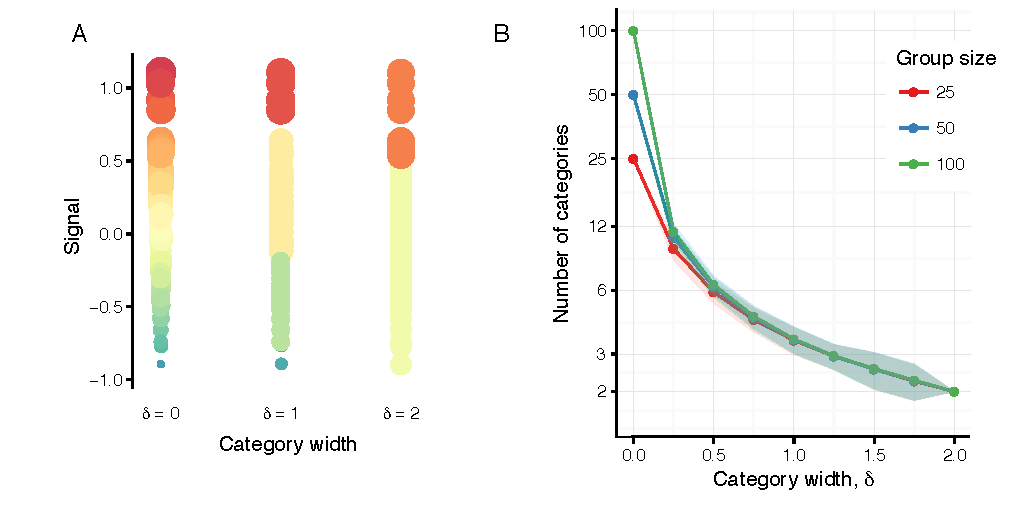
\includegraphics[width=6.85in]{figures/category_diagram.pdf}
\caption{\sffamily\small\textbf{As category width increases, the animals use fewer categories, each of which includes more animals.} 
In A we show how a given set of signals could be categorized using three different category widths ($\delta$). The three vertical lines of dots represent the same group, with the same set of signals $\{s_i\}$. Each dot represents an animal in the group and the vertical position of a dot represents the animal's signal. In each column, animals in the same category are represented by circles of the same size and color, indicated the average signal for animals in that category. The range of signals in a given category can be no more than $\delta$. In the left column, $\delta=0$ and there are $N=100$ categories. In the middle column, $\delta=1$ and there are four categories. In the right column, $\delta=2$ and there are two categories.  In B, we show how the number of categories an animal uses depends on the category width. For a given group size ($N$) and category width, we generated $5,000$ groups with signal values $\{s_i\}$ and categorized the group according to the procedure shown in A.  Category width is on the x-axis. The average number of categories across the $5,000$ groups is on the y-axis, which is on a logarithmic scale, with the color indicating group size. The shaded areas show this average plus or minus the standard deviation across the $5,000$ groups. When $\delta=0$ there are as many categories as there are animals in the group. When $\delta=2$, it is theoretically possible for all animals to be put into the same category, but this was never observed, and instead the animals were always put into $2$ categories. }
 \label{category_diagram}
\end{figure}

\begin{figure}
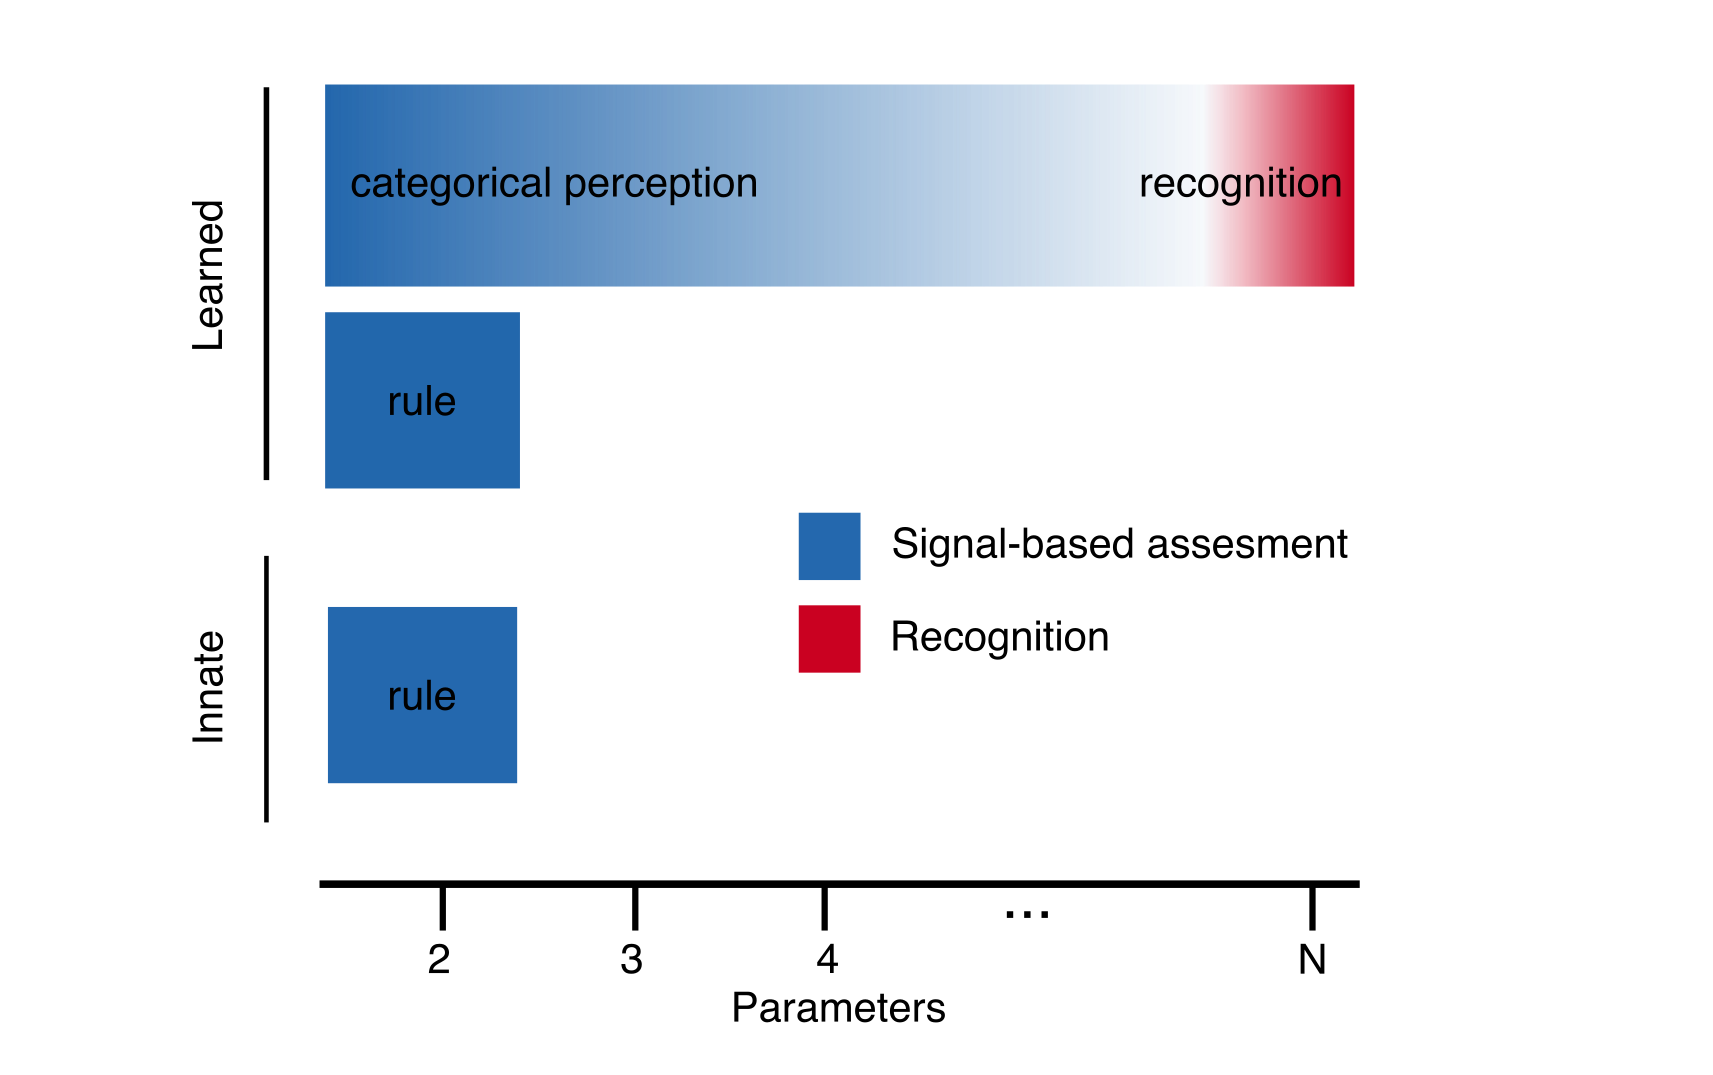
\includegraphics[width=6.85in]{figures/schematic_cropped.png}
\caption{\sffamily\small\textbf{Animals can use signals to infer the quality values of conspecifics.} They can do so using either a linear rule, which can be either learned or innate and which is determined by a slope and intercept, or categories, which can be coarse or fine. When there are as many categories as there are individuals in the group, categorical perception becomes individual recognition.}
\label{schematic}
\end{figure}

\begin{figure}
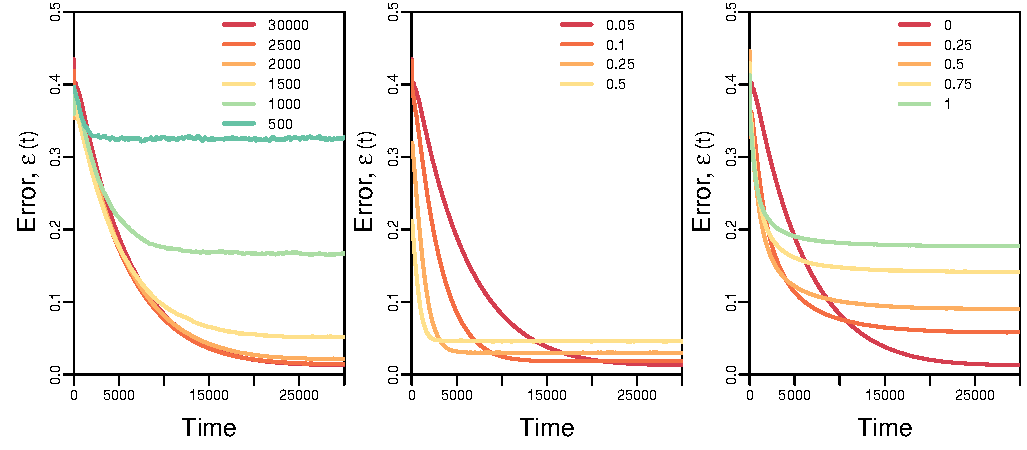
\includegraphics[width=6.85in]{figures/speed_accuracy_tradeoff.pdf}
\caption{\sffamily\small\textbf{As the animals learn, their errors decrease and eventually reach an equilibrium value.} Increasing the updating rate ($r$) or category width ($\delta$) helps the animals learn more quickly. When they have a long memory, this increases the equilibrium level of error, but when they have a short memory, it decreases the equilibrium level of error. In each panel, we show time ($t$, in number of interactions) on the x-axis and the average error in an animal's assessment of its peers ($\epsilon(t)$) on the y-axis. In each panel, light blue indicates animals using a learned rule, dark blue indicates animals using an innate rule, reddish colors indicates animals using recognition, and purple indicates animals using categorization. The points show the stopping time ($\tau$) at which error stops decreasing (not shown for the innate rule because there is no learning). In A and B, the different reddish curves represent different updating rates ($r$). In C and D, the red and purple curves represent different category widths ($\delta$). In the left column, memory window $w=2500$ and in the right column, memory window $w=500$. Parameters: unless the parameter is being varied $\delta=0$, $N=25$, $\rho=0.99$, $r=0.05$.}
\label{tradeoff}
\end{figure}

\begin{figure}
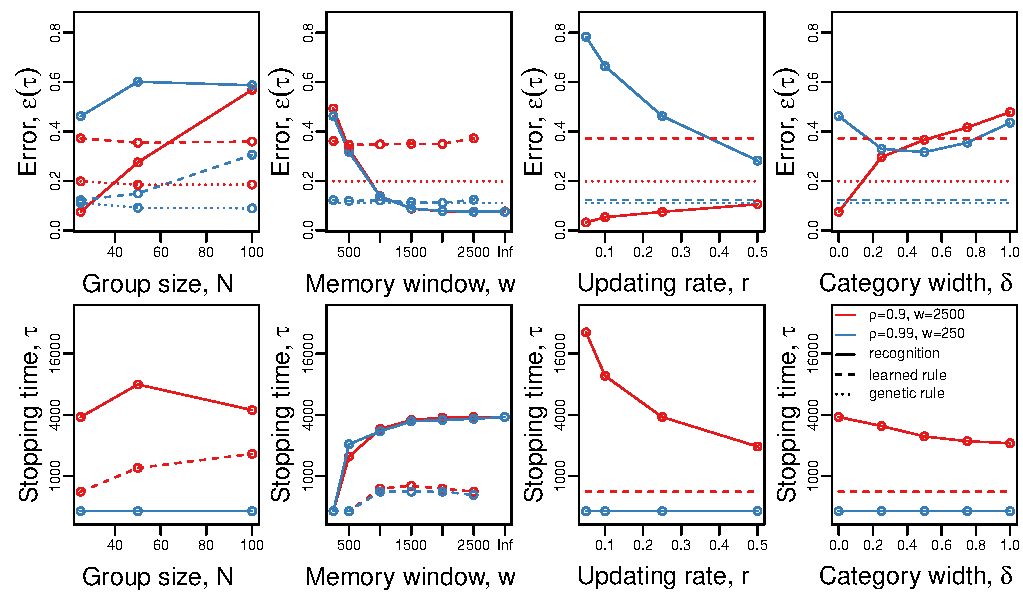
\includegraphics[width=6.85in]{figures/parameters_exploration.pdf}
\caption{\sffamily\small\textbf{Animals can learn about their peers with smaller errors when they have signals that are highly correlated with quality, live in small groups, and have long memory windows, and when errors are costly.} Here we show (A-D) average error ($\epsilon(\tau)$) and (E-H) stopping time ($\tau$) as a function of signal-quality correlation ($\rho$), group size ($N$), memory window ($w$), and cost of errors ($c$). Stopping time is on a logarithmic scale. In each panel, light blue curves show animals using a learned rule, dark blue curves show animals using a innate rule, red curves show animals using recognition ($\delta=0$), and purple curves show animals using categorization (with $\delta=0.25$). We do not show stopping time for animals using the innate rule because there is no learning involved.  The solid curves correspond to groups in which the signal-quality correlation $\rho=0.99$ and the dashed curves correspond to groups in which the signal-quality correlation $\rho=0.9$ (except in A and E, where we explicitly vary $\rho$). There are no dashed red curves because $\rho$ does not affect animals using recognition. The dark blue lines in G, and H do not have any points because these parameters, $w$ and $c$, do not affect the innate rule, so we show the value of $\epsilon(\tau)$ for animals using an innate rule as baseline to which we can compare the other strategies. 'All' means that the animals can remember all of their interactions. We do not run the model of the learned rule with memory window equal to 'All' because finding the regression of perceived quality values on observed signals values becomes unfeasible. Parameters: unless the parameter is being varied $c=1$, $N=25$, $r=0.5$, $w=2500$.}
\label{parameters}
\end{figure}

\begin{figure}
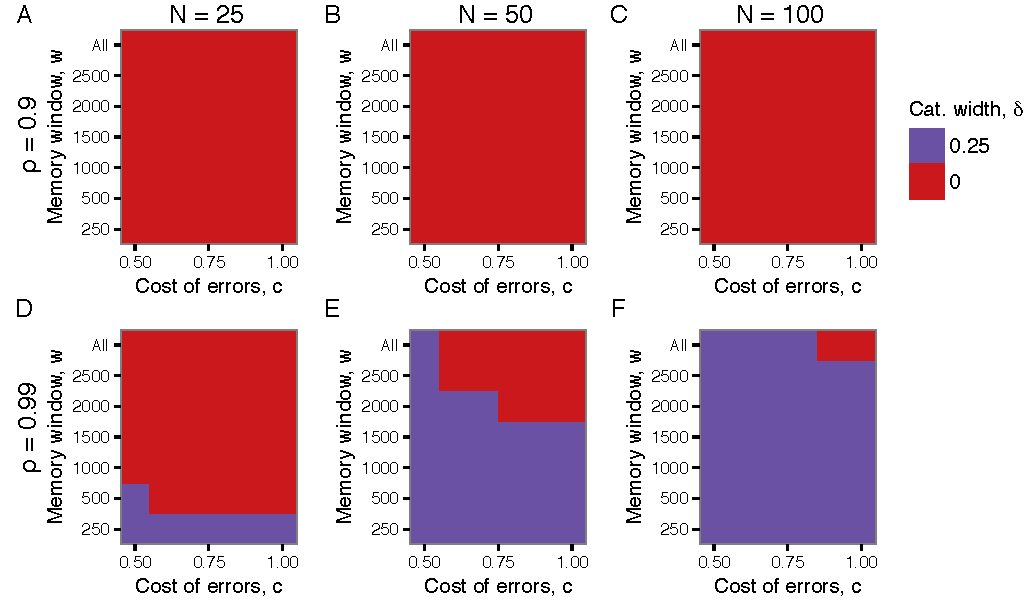
\includegraphics[width=6.85in]{figures/strategies_heat_maps.pdf}
\caption{\sffamily\small\textbf{Categorization is the better than recognition when animals live in large groups, have short memories, when the signal-quality correlation is high, and when errors are not very costly.} Here we show how the optimal category width ($\delta$), as a function of the cost of errors ($c$) and memory window ($w$). The optimal category width is the value of $\delta$ that minimizes the costs incurred from the combination of error and learning time. We concurrently find the value of $r$ that minimizes costs, as shown in Figure \ref{l}. 'All' means that the animals can remember all of their interactions. In the first column, group size $N=25$, in the second column $N=50$, and in the third column $N=100$. Parameters: $\rho=0.99$. }
\label{opt_delta}
\end{figure}


\begin{figure}
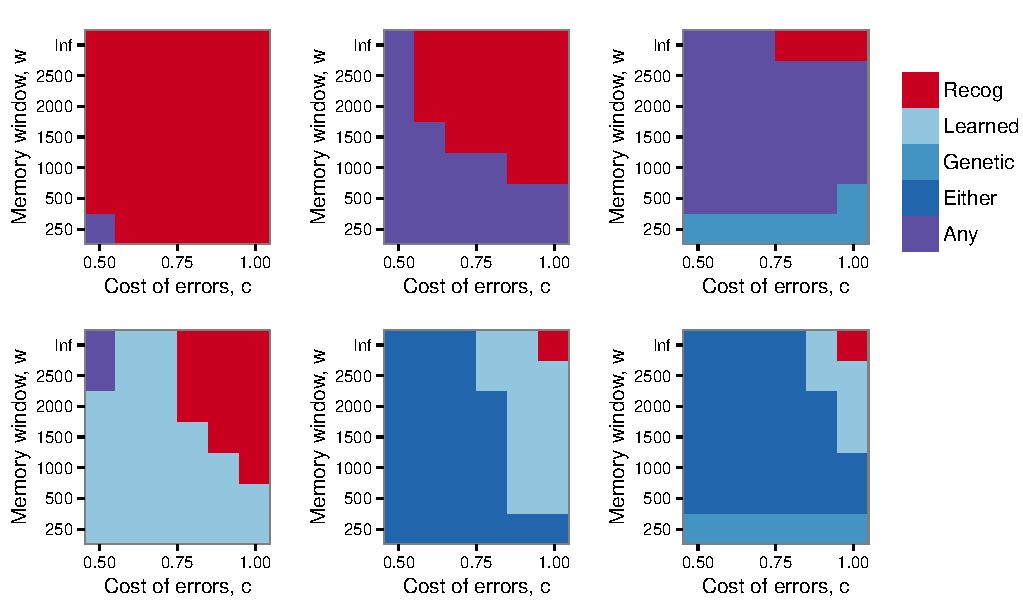
\includegraphics[width=6.85in]{figures/best_type_of_learning.pdf}
\caption{\sffamily\small\textbf{A rule is the best assessment strategy when animals live in large groups and have short memories, when the signal-quality correlation is high, and when errors are not very costly.} Here we show which of the three assessment strategies---recognition, a learned rule, or a innate rule---is the least costly, as a function of the cost of errors ($c$) and memory window ($w$). Red indicates recognition is the least costly. Light blue indicates a learned rule is the best strategy. Intermediate blue indicates a innate rule is the best strategy. Dark blue indicates the two rules are essentially equally costly and less costly than recognition. Grey indicates the three strategies are all essentially equally costly. (Strategies are classified as equivalent if their costs are within $0.05$ of each other.) Using categorization is never the least costly strategy. Animals using recognition are using the optimal stopping time ($\tau$), updating rate ($r$), and category width ($\delta=0$), as shown in Figures \ref{time}, \ref{l}, and \ref{opt_delta}, respectively, and animals using a learned rule are using the optimal stopping time. 'All' means that the animals can remember all of their interactions. We do not run the model of the learned rule with memory window equal to 'All' because finding the regression of perceived quality values on observed signals values becomes unfeasible. Instead, we assume that animals using the learned rule can remember at most $2500$ time steps, which is a valid approximation because memory widnwo does not strongly affect the learned rule. In the first column $N=25$, in the middle column, $N=50$, and in the right column $N=100$. In the first row $\rho=0.9$ and in the second row $\rho=0.99$.}
\label{best}
\end{figure}

%
\begin {table}[ht]
\caption {Description of variables} \label{tab:vars} 
\begin{tabular}{cl}

 Variables & Description of variables \\
\midrule 
$a_{ij}(t)$ & animal $i$'s assessment of animal $j$ at time $t$ \\
$C(t)$ & total cost of learning \\ 
$c$ & cost of errors, whereas $1-c$ is the cost of spending time learning \\ 
$\delta$ & category width (values near 0 = higher discriminatory ability, $\delta=0 \approx$ individual recognition)\\
$e_{ij}(t)$ & error of animal $i$ about animal $j$ at time $t$\\
$\epsilon(t)$ & average error of all animals in all groups at time $t$ \\
$N$ & number of animals in group (small=25, medium=50, large=100)\\ 
$\mathscr{O}_i(t)$ & set of animals about whom $i$ has an opinion at time $t$\\
$q_j$ & quality of animal $j$ \\ 
$\hat{q}_j$ & noisy information about the quality of animal $j$, $\hat{q}_j=q_j+\xi$ \\
$r$ & updating rate (values near 0 = very fast updating rates)\\
$\rho$ & sample correlation between quality and signal (high=0.9, almost perfect=0.99)\\
$s_j$ & quality signal of animal $j$ \\ 
$\sigma_\xi$ & standard deviation of noise in opinion updating during interaction, set to $0.1$ \\
$\sigma_\text{q}$ & standard deviation of quality values, set to $0.5$ \\
$T$ & total number of interactions, set to $30,000$ \\
$\tau$ & stopping time \\
$w$ & memory window (values near 0 = very short-term memory)\\
$\xi$ & noise in the information animals get about each other's quality through interacting
\end{tabular}
\end {table}



\newpage
\begin {table}[ht]
\renewcommand*{\arraystretch}{1.4}
\caption {Description of variables} \label{tab:vars2} 
\begin{tabular}[t]{ |c|c|l| }
  \hline
  \multirow{6}{*}{\rotatebox[origin=c]{90}{\parbox{2cm}{\centering Interaction \\ parameters}}} 
  & $q_j$ 			& Quality of animal $j$ \\   
  & $\hat{q}_j$ 		& Noisy information about the quality of animal $j$, $\hat{q}_j=q_j+\xi$ \\ 
  & $s_j$ 			& Signal of animal $j$ \\ 
  & $\sigma_\xi$ 	& Standard deviation of noise in opinion updating during interaction, set to $0.1$ \\
  & $\sigma_\text{q}$ & Standard deviation of quality values, set to $0.5$ \\
  & $T$ 			& Total number of interactions, set to $30,000$ \\
  & $\xi$ 			& Noise in the information animals get about each other's quality through interacting \\
  \hline
  \multirow{5}{*}{\rotatebox[origin=c]{90}{\parbox{2cm}{\centering Assessment \\ parameters}}}
  & $c$ 				& Cost of errors, whereas $1-c$ is the cost of spending time learning \\ 
  & $\delta$ 	& Category width (ranges from $0$, meaning recognition, to $2$, where animals use $2$ categories)\\
 	& $N$ & Number of animals in group (can equal $25$, $50$, or $100$) \\
 	 & $r$ 		& Updating rate (range from $0.05$ to $0.5$)\\
  & $\rho$ 		& Sample correlation between quality and signal. (can equal $0.5$, $0.9$, or $0.99$) \\
  & $w$ 		& Memory window (ranges from $0$, meaning poor memory, to 'All', meaning every interaction)\\
  \hline
  \multirow{7}{*}{\rotatebox[origin=c]{90}{\parbox{2cm}{\centering Assessment \\ output}}} 
  & $a_{ij}(t)$ 		& Animal $i$'s assessment of animal $j$ at time $t$ \\
   & $C(t)$ 				& Total cost of learning \\ 
    & $e_{ij}(t)$ 		& Error of animal $i$ about animal $j$ at time $t$\\
  & $\epsilon(t)$ 		& Average error of all animals in all groups at time $t$ \\
  & $\mathscr{O}_i(t)$ 	& Set of animals about whom $i$ has an opinion at time $t$\\
  & $\tau$ 				& Stopping time \\

  \hline
\end{tabular}
\end {table}





%%%%%%%%%%%%%%%%%%%%%% FIGURES
%\clearpage
%\setcounter{figure}{0}

%\begin{figure}
%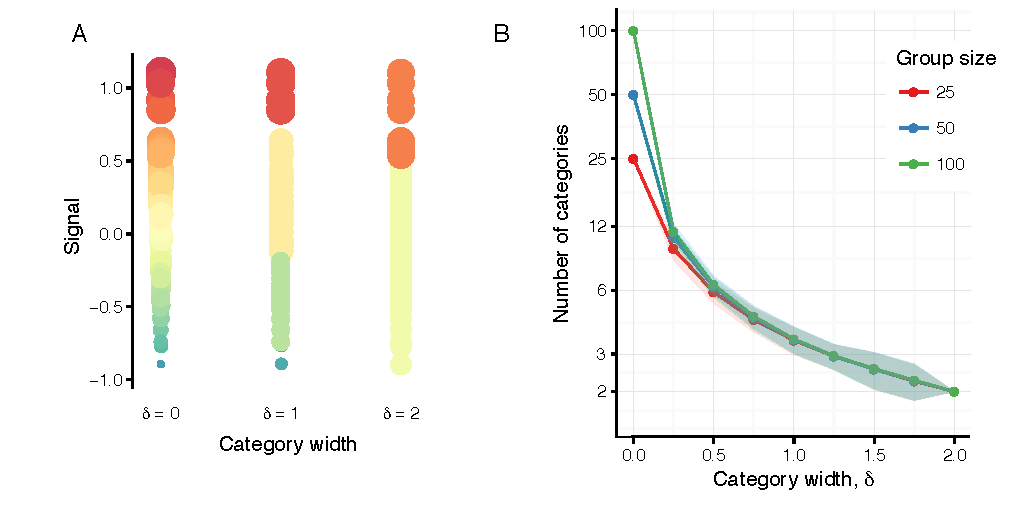
\includegraphics[width=6.85in]{figures/category_diagram.pdf}
%\caption{}
%\end{figure}

%\begin{figure}
%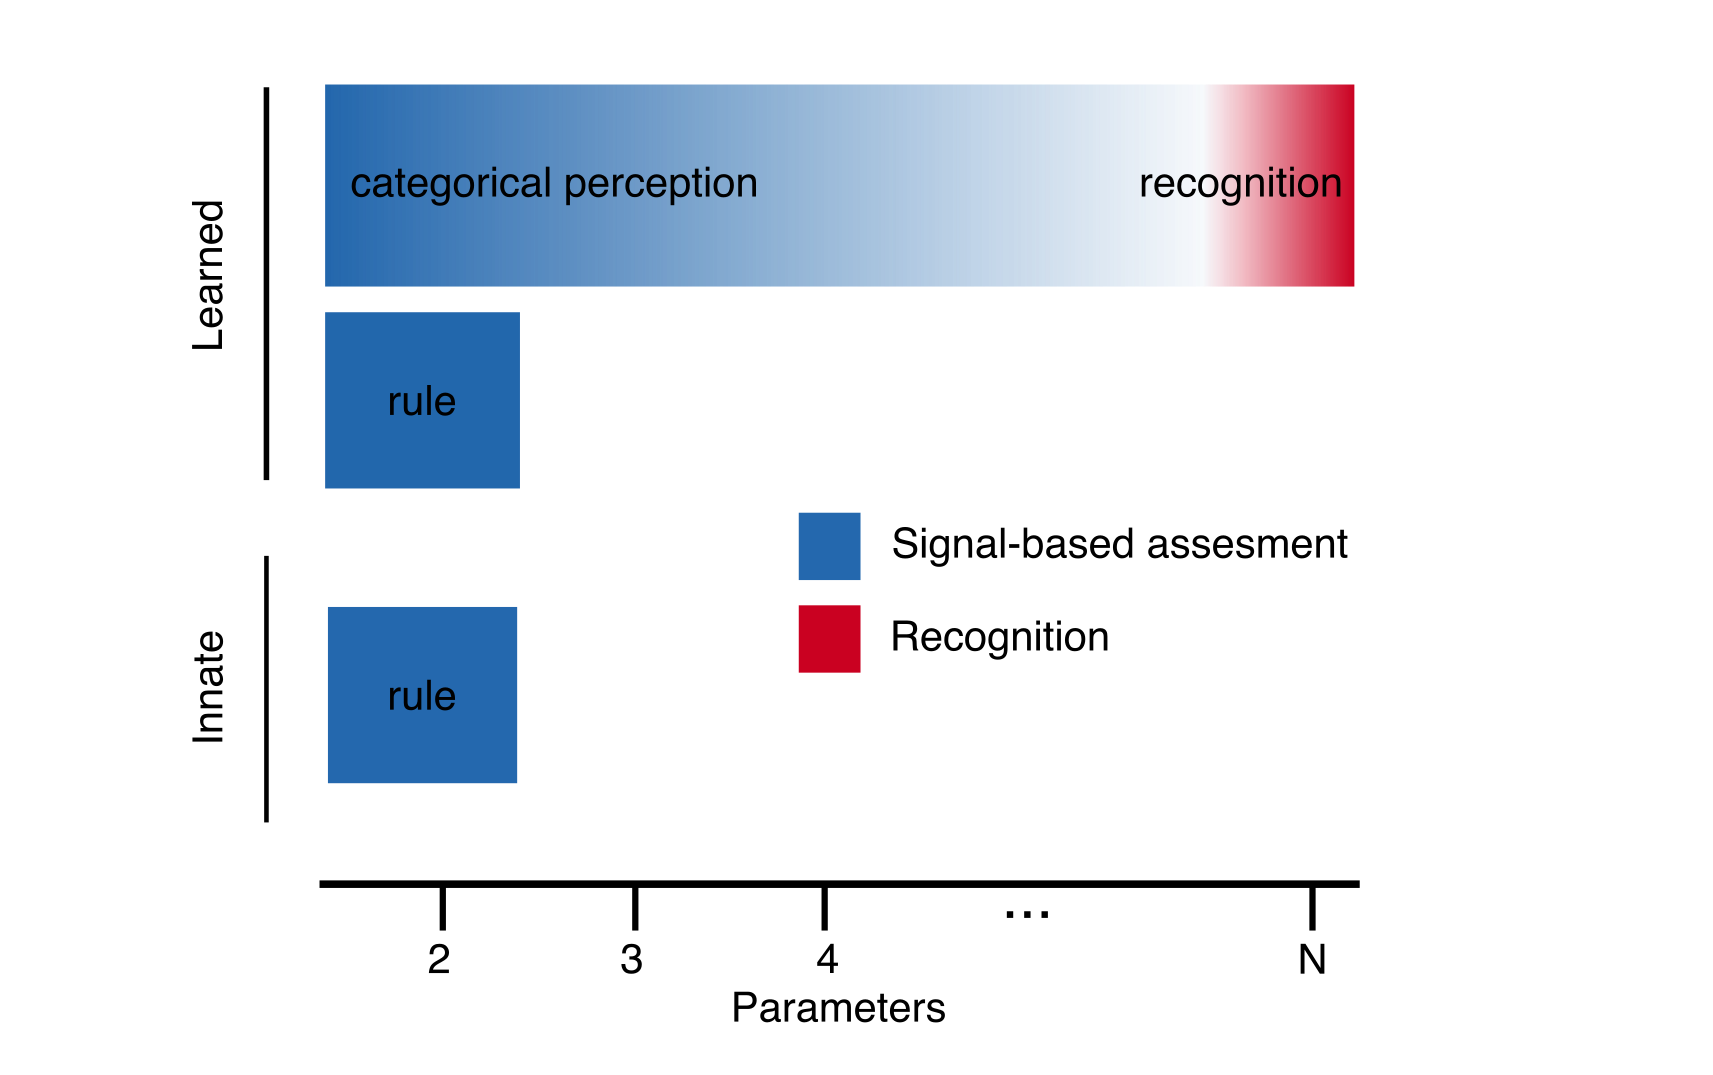
\includegraphics[width=6.85in]{figures/schematic_cropped.png}
%\caption{}
%\end{figure}

%\begin{figure}
%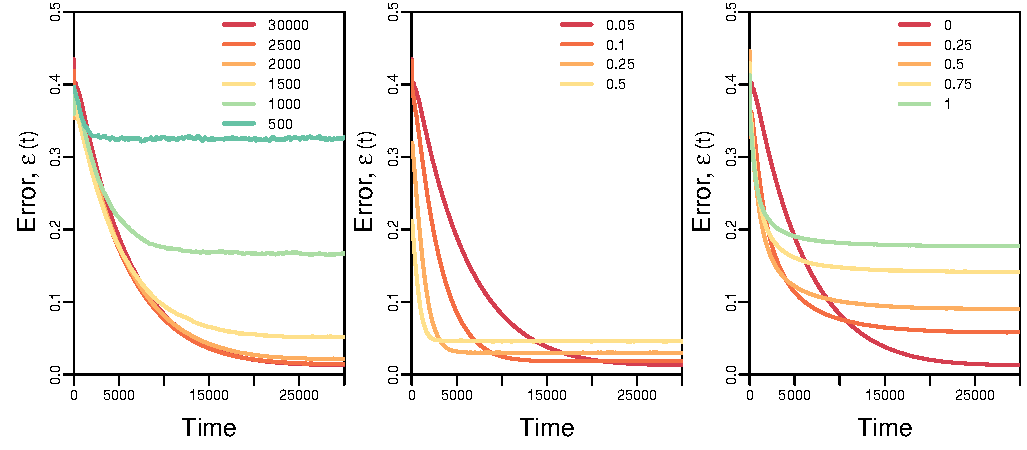
\includegraphics[width=6.85in]{figures/speed_accuracy_tradeoff.pdf}
%\caption{}
%\end{figure}

%\begin{figure}
%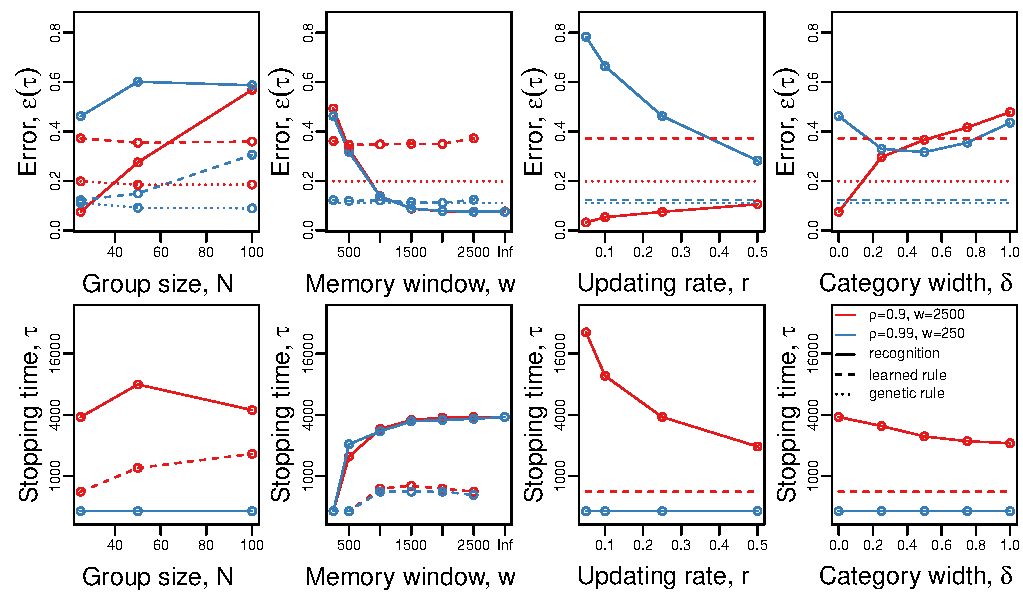
\includegraphics[width=6.85in]{figures/parameters_exploration.pdf}
%\caption{}
%\end{figure}


%\begin{figure}
%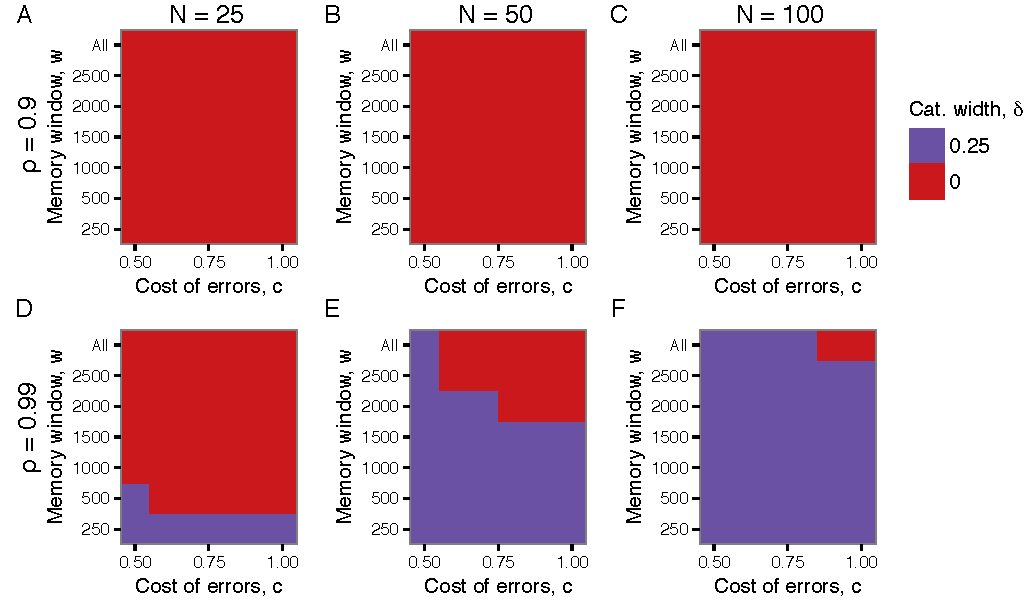
\includegraphics[width=6.85in]{figures/strategies_heat_maps.pdf}
%\caption{}
%\end{figure}


%\begin{figure}
%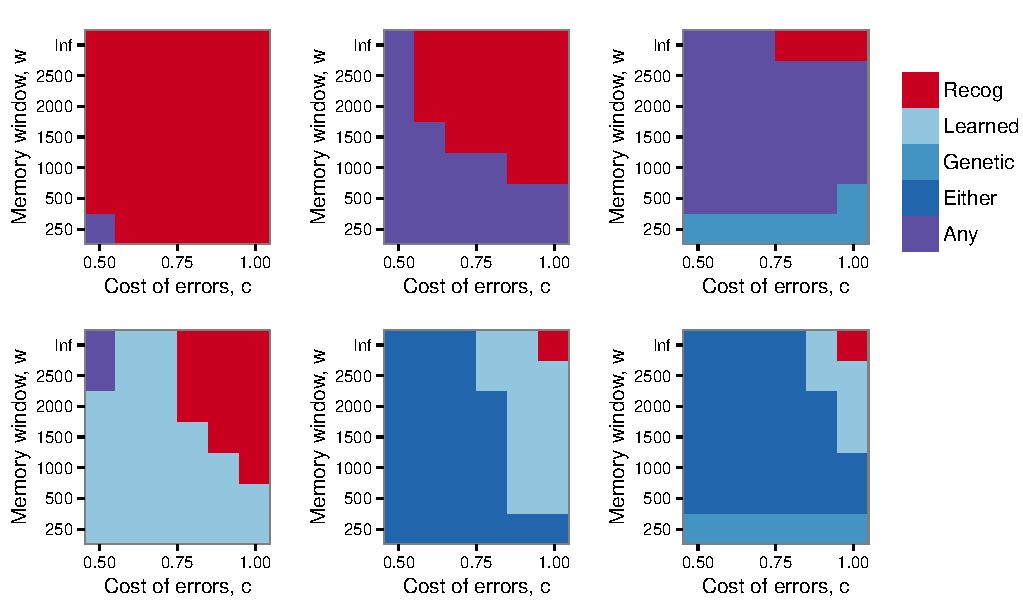
\includegraphics[width=6.85in]{figures/best_type_of_learning.pdf}
%\caption{}
%\end{figure}

\clearpage{}
\newpage{}
\renewcommand{\thesection}{}
\section{Supporting information}
\renewcommand{\thesection}{S}
\renewcommand{\thesubsection}{S\arabic{subsection}}
\renewcommand{\theequation}{S\arabic{equation}}
\renewcommand{\thetable}{S\arabic{table}}
\renewcommand{\thefigure}{S\arabic{figure}}
\setcounter{equation}{0}  
\setcounter{figure}{0}
\setcounter{table}{0}

\begin{figure}[ht]
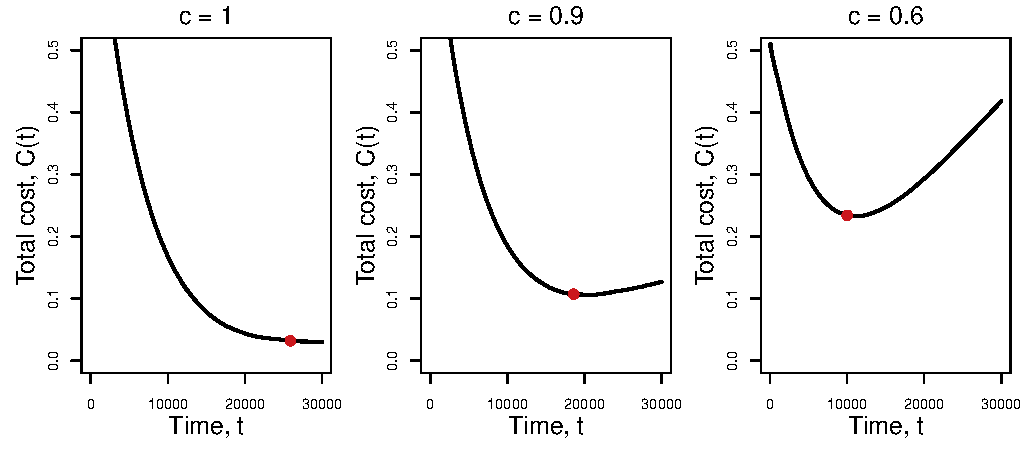
\includegraphics[width=6.85in]{figures/stopping_time.pdf}
\caption{\sffamily\small\textbf{As the cost of errors decreases and the cost of learning time increases, animals should stop learning earlier.} Here we show how we calculate stopping time ($\tau$). In each panel, time in number of interactions ($t$) is on the x-axis and the total cost $C(t)$ is on the y-axis. In A, the cost of errors $c=1$: all that matters is error and the total cost $C(t)$ is equal to $2$ times the average error $\epsilon(t)$. In B, the cost of errors $c=0.9$ and in C, the cost of errors $c=0.6$: in each case, as time goes on, the animals incur costs from their interactions. In each panel, the stopping time $\tau$ is shown with the red point: this is the number of interactions at which the cost $C$ stops decreasing and either plateaus or starts to increase. Parameters: $\delta=0$, $N=25$, $\rho=0.9$, $r=0.05$, $w=2500$.)
}
\label{tau}
\end{figure}


\begin{figure}[ht]
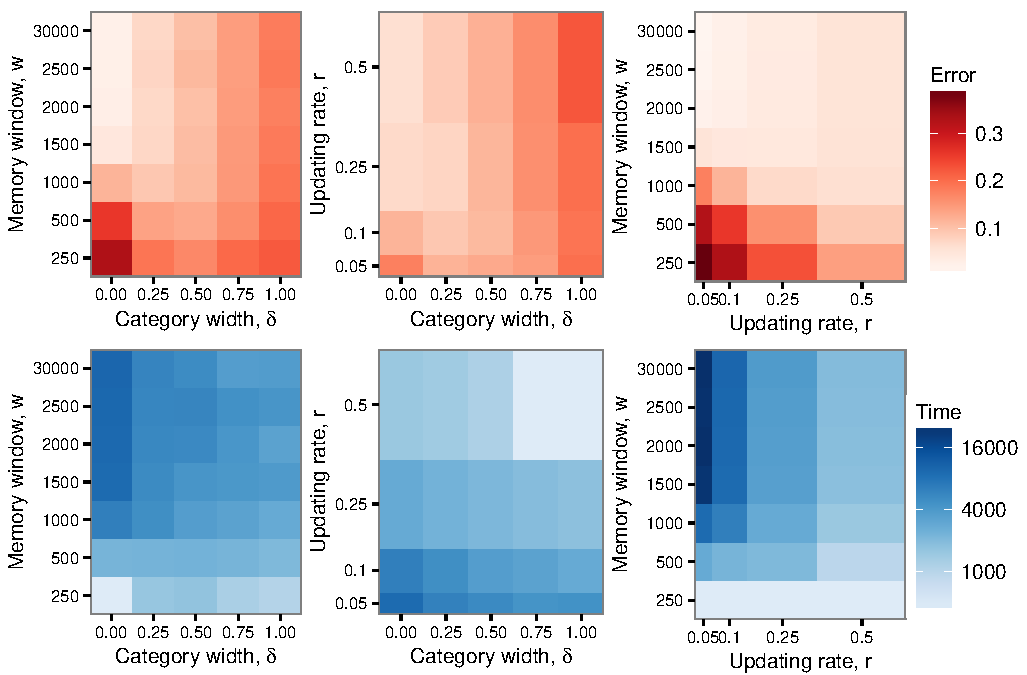
\includegraphics[width=6.85in]{figures/parameters_interactions_full.pdf}
\caption{\sffamily\small\textbf{Memory window, updating rate, and category width interact in their effects on how quickly and accurately animals using categorization can learn.}
Here we show stopping time ($\tau$) (A-C) and average error ($\epsilon(\tau)$) (D-F) for animals using categorization as a function of two parameters. Stopping time is on a logarithmic scale. Increasing memory window increases stopping time (A and C) and decreases error (D and F). Increasing category width decreases stopping time (A and B). Intermediate category widths minimize error when memory and updating rate are low, but otherwise category width $\delta=0$ minimizes error (D and E). Increasing updating rate decreases stopping time (B and C). When memory window is low, increasing updating rate decreases error, but when memory window is high, increasing updating rate \emph{increases} error (F). Parameters: unless the parameter is being varied $\delta = 0$, $N=25$, $\rho=0.99$, $w=1000$, $r=0.1$. 
}
\label{interactions}
\end{figure}

\begin{figure}
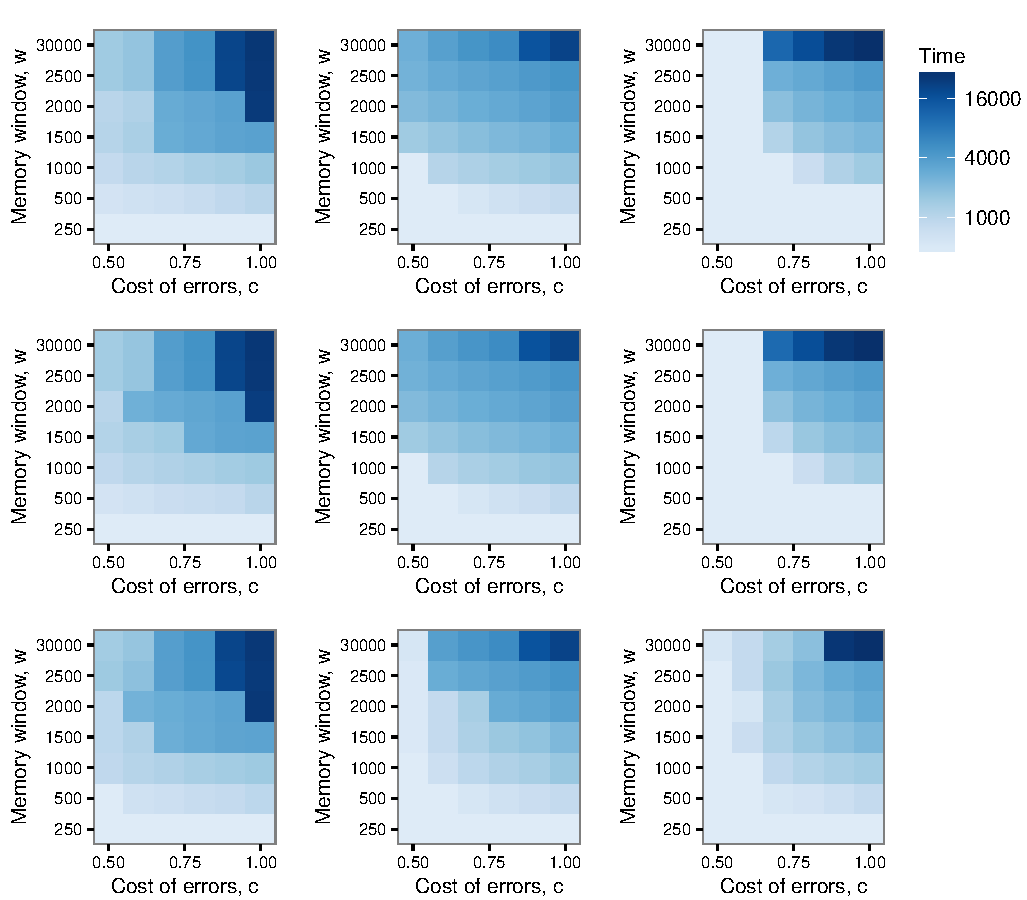
\includegraphics[width=6.85in]{figures/time_heat_maps.pdf}
\caption{\sffamily\small\textbf{} Here we show how the optimal stopping time ($\tau$) animals using categorization depends on the cost of errors ($c$) and memory window ($w$). Stopping time is on a logarithmic scale. In the first column $N=25$, in the middle column $N=50$, and in the right column $N=100$. In the first row $\rho=0.5$, in the second row $\rho=0.9$ and in the third row $\rho=0.99$. The animals are also using the optimal updating rate ($r$) and category width ($\delta$), which are shown in Figures \ref{opt_delta} and \ref{l}.}
\label{time}
\end{figure}

%\begin{figure}
%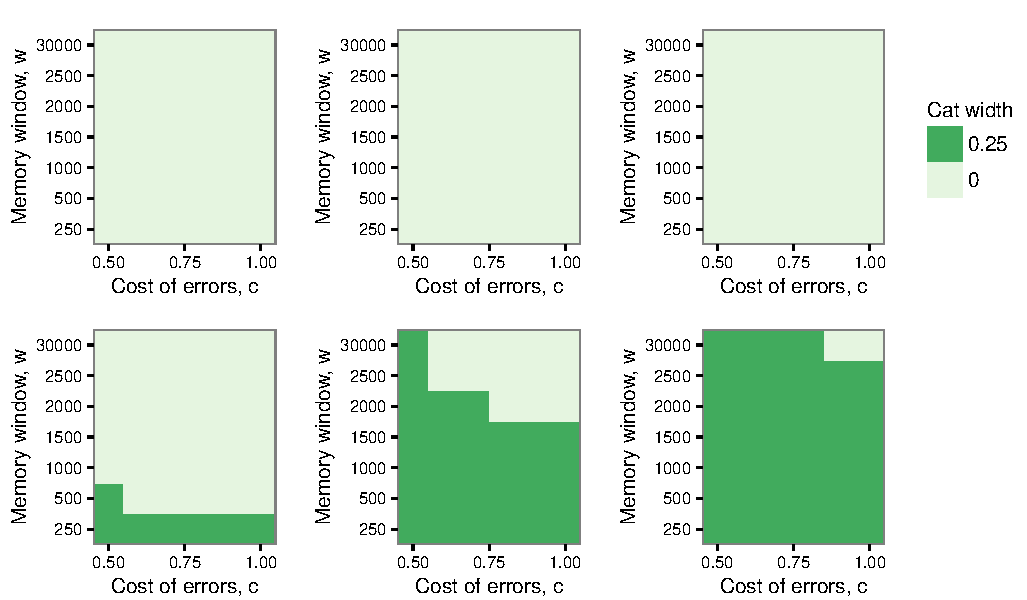
\includegraphics[width=6.85in]{figures/delta_heat_maps.pdf}
%\caption{\sffamily\small\textbf{Categorical recognition is better than individual recognition when animals live in large groups and have short memory windows and when the signal-quality correlation is very high.} Here we show how the optimal category width ($\delta$) animals using categorization depends on the cost of errors ($c$) and memory window ($w$). In the first column $N=25$, in the middle column $N=50$, and in the right column $N=100$. In the first row $\rho=0.5$, in the second row $\rho=0.9$, and in the third row $\rho=0.99$. The animals are also using the optimal stopping time ($\tau$) and updating rate ($r$), which are shown in Figures \ref{time} and \ref{l}.}
%\label{delta}
%\end{figure}

\begin{figure}
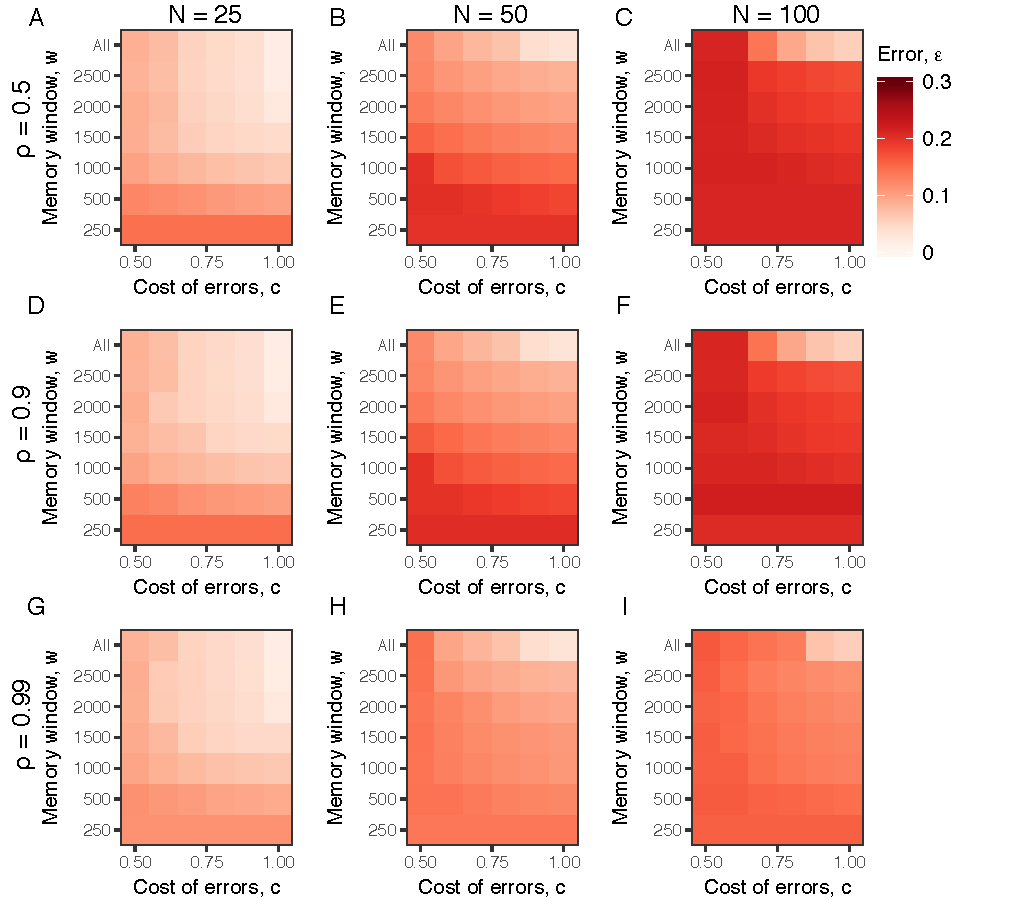
\includegraphics[width=6.85in]{figures/error_heat_maps.pdf}
\caption{\sffamily\small\textbf{} Here we show how the average error ($\epsilon(\tau)$) of animals using categorization depends on the cost of errors ($c$) and memory window ($w$). In the first column $N=25$, in the middle column $N=50$, and in the right column $N=100$. In the first  row $\rho=0.5$, in the second row $\rho=0.9$ and in the third row $\rho=0.99$. The animals are using optimal stopping time ($\tau$), updating rate ($r$), and category width ($\delta$), as shown in Figures \ref{time}, \ref{l}, and \ref{opt_delta}, respectively. }
\label{error}
\end{figure}

\begin{figure}
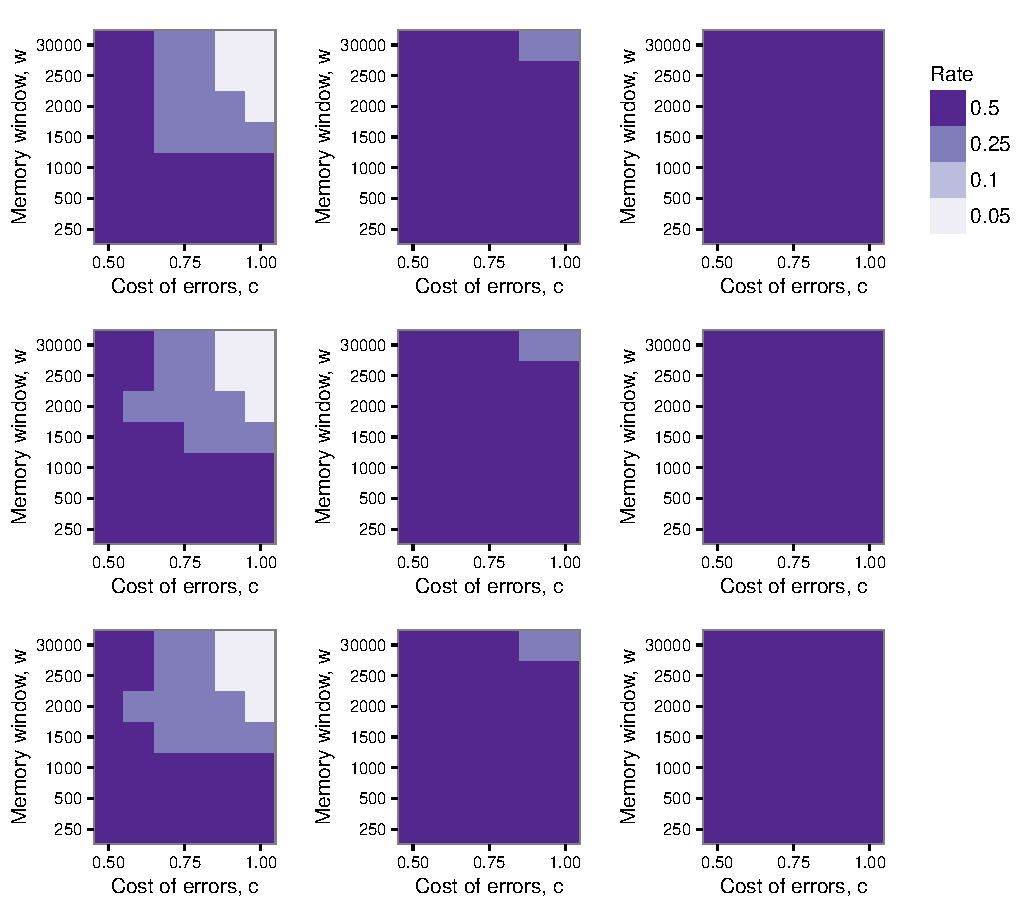
\includegraphics[width=6.85in]{figures/l_heat_maps.pdf}
\caption{\sffamily\small\textbf{A high updating rate is better than a low updating rate when animals live in large groups and have short memory windows.} Here we show how the optimal updating rate ($r$) animals using categorization depends on the cost of errors ($c$) and memory window ($w$). In the first column $N=25$, in the middle column $N=50$, and in the right column $N=100$. In the first row $\rho=0.5$, in the second row $\rho=0.9$, and in the third row $\rho=0.99$. The animals are also using the optimal stopping time ($\tau$) and category width ($\delta$), which are shown in Figures \ref{time} and \ref{opt_delta} respectively.}
\label{l}
\end{figure} 

%\begin{figure}
%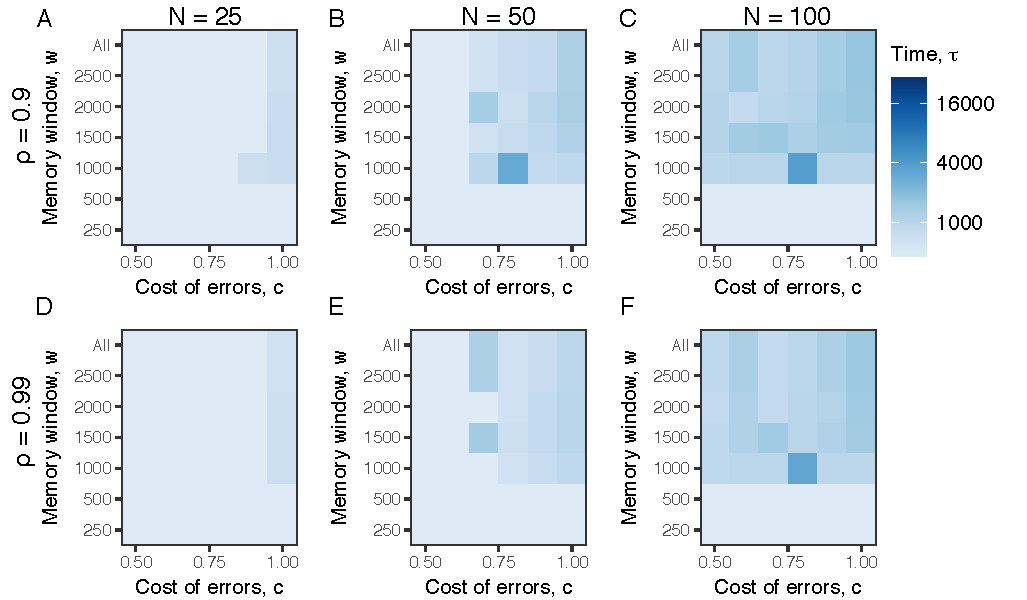
\includegraphics[width=6.85in]{figures/time_heat_maps_rule.pdf}
%\caption{\sffamily\small\textbf{} Here we show how the optimal stopping time ($\tau$) for animals using a learned rule depends on the cost of errors ($c$) and memory window ($w$). Stopping time is on a logarithmic scale. In the first column $N=25$, in the middle column $N=50$, and in the right column $N=100$. In the first row $\rho=0.9$ and in the second row $\rho=0.99$. }
%\label{time_rule}
%\end{figure}

%\begin{figure}
%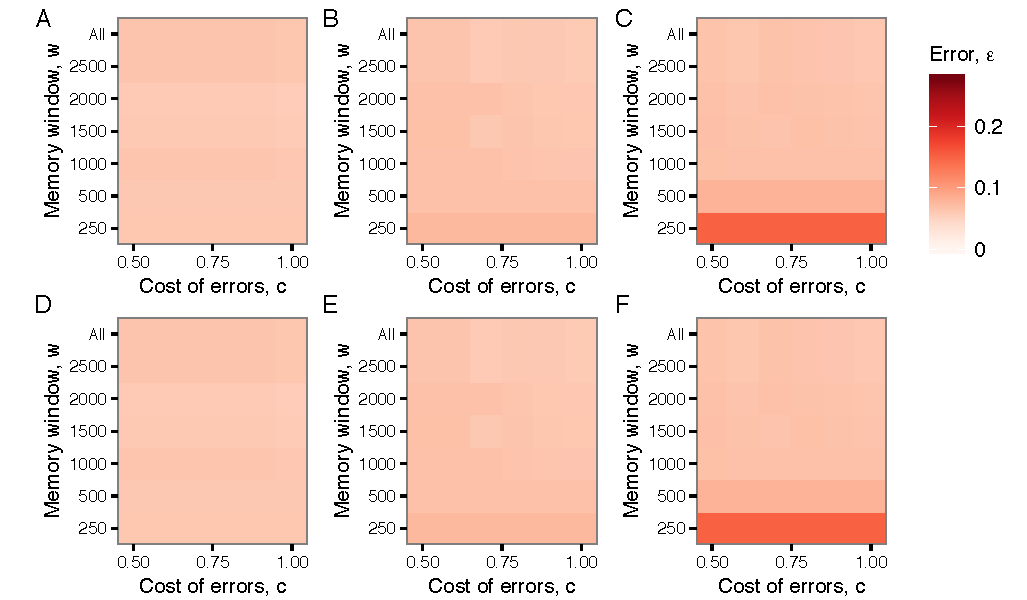
\includegraphics[width=6.85in]{figures/error_heat_maps_rule.pdf}
%\caption{\sffamily\small\textbf{} Here we show how the average error ($\epsilon(\tau)$) of animals using a learned rule with optimal stopping time ($\tau$) (shown in Figure \ref{time_rule}) depends on the cost of errors ($c$) and memory window ($w$). In the first column $N=25$, in the middle column $N=50$, and in the right column $N=100$. In the first  row $\rho=0.9$ and in the second row $\rho=0.99$.}
%\label{error_rule}
%\end{figure}

\begin{figure}
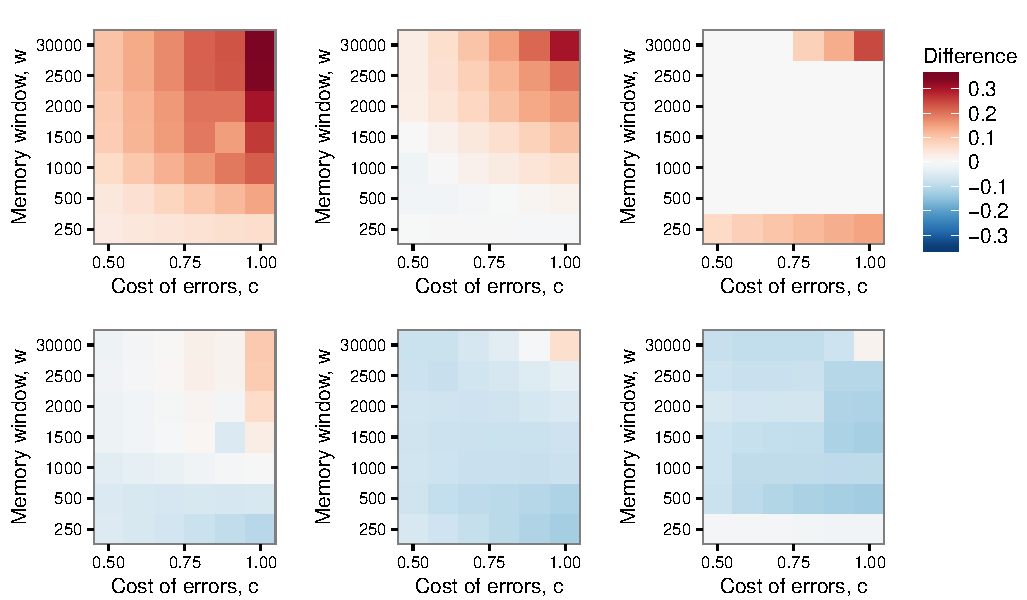
\includegraphics[width=6.85in]{figures/recog_vs_learned_rule.pdf}
\caption{\sffamily\small\textbf{A learned rule is less costly than recognition (with optimized learning strategies) when animals live in large groups and have short memories and when the signal-quality correlation is high.} In each panel, we show the difference in overall costs between recognition and a learned rule as a function of the cost of errors ($c$) and memory window ($w$). Blue indicates a learned rule is less costly and red indicates recognition is less costly. The animals using recognition are using the optimal stopping time ($\tau$), updating rate ($r$), and category width ($\delta$). In the first column $N=25$, in the middle column, $N=50$, and in the right column $N=100$. In the first row $\rho=0.9$ and in the second row $\rho=0.99$.}
\label{comparison}
\end{figure}

\begin{table}
\caption{\label{corr_examples} Examples of the correlation between a badge and a measure of fitness.}
\begin{tabular}{lllll}
Species & Badge & Measure of fitness & Correlation & Reference
\\\hline paper wasp & percent black on face & head width & $r^2=0.36$, for wasps  & Tibbetts \& Dale 2004
\\ & & & with $\geq 2$ black spots
\\ & ``badge brokenness" & dominance & $r^2=.105$ & Tibbetts \& Dale 2004
\\ \hline house sparrow & size of black bib & physical condition & $r=0.379$ & Veiga 1993
\\ \hline swamp sparrow & size of rusty cap & parental investment & $r^2=0.33$ & Olsen et al. 2010
\\ & size of black forehead & aggression & $r^2=0.41$ & Olsen et al. 2010
\end{tabular}
\end{table}

\end{document}
